% ------------------------------------------------------------------------
% ------------------------------------------------------------------------
% Modelo de TCC do curso de Engenharia de Controle e Automação - UFSC/Campus Blumenau
% Autor: Ciro André Pitz
% Revisão: Brenda Teresa Porto de Matos
% O presente modelo foi obtido a partir do modelo desenvolvido por Alisson Lopes Furlani disponível na BU/UFSC.
% ------------------------------------------------------------------------
% ------------------------------------------------------------------------

\documentclass[
12pt,				% tamanho da fonte
%openright,			% capítulos começam em pág ímpar (insere página vazia caso preciso)
oneside,			% para impressão no anverso. Oposto a twoside
a4paper,			% tamanho do papel. 
chapter=TITLE,		% títulos de capítulos convertidos em letras maiúsculas
section=TITLE,		% títulos de seções convertidos em letras maiúsculas
%subsection=TITLE,	% títulos de subseções convertidos em letras maiúsculas
%subsubsection=TITLE,% títulos de subsubseções convertidos em letras maiúsculas
% -- opções do pacote babel --
english,			% idioma adicional para hifenização
brazil				% o último idioma é o principal do documento
]{abntex2}

\usepackage{configs/eca_ufsc_bnu} % personalização da ABNTEX2 
\addbibresource{pos_textual/referencias.bib} % Seus arquivos de referências

%---------------------------------------------------------------------------------------------
%--------- DADOS BÁSICOS DO TCC (Preencher todos) -------------------------------------
%---------------------------------------------------------------------------------------------
%Substituir 'Nome completo do autor' pelo seu nome.
\autor{André Carpinteiro do Amaral \\ Jefferson de Morais Correia \\ Marcelo Gervazoni Carbonera}
% FIXME Substituir 'Título do trabalho' pelo título da trabalho.
\titulo{Previsão de disponibilidade de água no Sistema Cantareira}
% Substituir 'Subtítulo (se houver)' pelo subtítulo da trabalho. 
% Se não houver subtítulo, basta comentar o texto (usando o símbolo de porcentagem).
%\subtitulo{subtítulo (se houver)}
% Substituir 'Orientador' pelo nome do seu orientador.
% \orientador{Profª. Dra. Marilde Santos}
% Se for orientado por uma mulher, comente a linha acima e descomente a linha a seguir.
\orientador[Orientadora]{Profª. Dra. Marilde Terezinha Prado Santos}
% Substituir 'XXXXXX' pelo nome do seu  coorientador. Caso não tenha coorientador, comente a linha a seguir.
% \coorientador{Profª. Dra. Marilde Santos}
% Se for coorientado por uma mulher, comente a linha acima e descomente a linha a seguir.
%\coorientador[Coorientadora]{Profª. Dra. Marilde Santos}
\dia{11}
\mes{Janeiro}
\ano{2026}
\local{São Carlos/SP}
\formacao{Especialista em MBA em Machine Learning in Production}
% Se for mulher, comente a linha acima e descomente a linha a seguir.
%\formacao{Engenheira de Controle e Automação}
\bancaa{Profª. Dra. Marilde  Terezinha Prado Santos} %Primeiro membro da banca (normalmente o orientador).
\bancab{Prof. Segundo, Dr.} %Segundo membro da banca
\bancac{Prof. Terceiro, Dr.} %Terceiro membro da banca

%Resumo e palavras-chave do trabalho
\resumotcc{A gestão eficiente dos recursos hídricos é fundamental para garantir o abastecimento de água e manter a sustentabilidade socioeconômica da população. O Sistema Cantareira destaca-se como um dos principais produtores de água da Região Metropolitana de São Paulo, sendo responsável pelo abastecimento de aproximadamente 46\% da população. Diante da relevânciadesse sistema e da recorrência de eventos climáticos extremos, torna-se essencial o desenvolvimento de ferramentas capazes de antecipar cenários críticos de disponibilidade hídrica. Este trabalho tem como objetivo contribuir para a melhoria da gestão do Sistema Cantareira por meio da previsão da disponibilidade de água, utilizando técnicas de análise de séries temporais e aprendizado de máquina. A proposta consiste na construção de uma arquitetura capaz de coletar e tratar automaticamente dados operacionais disponibilizados diariamente pela SABESP, modelar o comportamento do volume útil (\%) do sistema e gerar previsões em um horizonte temporal definido. A metodologia adotada baseia-se em uma abordagem híbrida de decomposição da série temporal, na qual os componentes de tendência e sazonalidade são modelados por algoritmos lineares, enquanto as oscilações cíclicas e não lineares são capturadas por modelos de aprendizado de máquina clássicos, treinados sobre os resíduos. Variáveis exógenas, como vazão natural e vazão jusante, são incorporadas ao processo para representar a dinâmica física do sistema. As previsões resultantes são apresentadas por meio de visualizações que permitem identificar, de forma antecipada, a aproximação de níveis críticos de armazenamento, em especial o limiar de 30\% do volume útil, associado a estados de alerta e restrição. Além disso, há parâmetros a serem testados caso o desempenho do modelo caia com o passar do tempo, incorporando o retreino e avaliação de novos modelos como parte do ciclo de vida de Machine Learning do projeto.}
\palavraschave{Séries temporais; Recursos hídricos; Sistema Cantareira; Aprendizado de máquina; Previsão de disponibilidade de água.}

%Abstract e keywords do trabalho
\abstracttcc{Efficient management of water resources is fundamental to ensure water supply and maintain the socioeconomic sustainability of the population. The Cantareira System stands out as one of the main water producers for the São Paulo Metropolitan Region, responsible for supplying approximately 46\% of the population. Given the significance of this system and the recurrence of extreme weather events, the development of tools capable of anticipating critical scenarios of water availability becomes essential. This study aims to contribute to improving the management of the Cantareira System through water availability forecasting, utilizing time series analysis and machine learning techniques. The proposal involves building an architecture capable of automatically collecting and processing operational data made available daily by SABESP, modeling the behavior of the system's useful volume (\%), and generating forecasts within a defined time horizon.The adopted methodology is based on a hybrid time series decomposition approach, in which trend and seasonality components are modeled using linear algorithms, while cyclical and non-linear oscillations are captured by classic machine learning models trained on residuals. Exogenous variables, such as natural flow (inflow) and downstream flow (outflow), are incorporated into the process to represent the physical dynamics of the system. The resulting forecasts are presented through visualizations that allow for the early identification of approaching critical storage levels, specifically the 30\% useful volume threshold associated with alert and restriction states. Furthermore, parameters are established to be tested should model performance degrade over time, incorporating retraining and the evaluation of new models as part of the project's Machine Learning lifecycle.}
\keywords{Time series; Water resources; Cantareira System; Machine learning; Water availability forecasting.}

%Agradecimentos (opcional). Caso não queira inserir, deixe em branco (\agradecimentostcc{} )
\agradecimentostcc{Agradecemos aos professores das disciplinas do MBA, especialmente a Marilde por ter nos acompanhado ao longo desses 18 meses e deixado tudo mais tranquilo. Agradecemos também a nossos pais, familiares e amigos que nos apoiaram e ajudaram a tornar possível a execução deste trabalho.}

%Epígrafe (opcional). Caso não queira inserir, deixe em branco (\epigrafetcc{} )
\epigrafetcc{}

%Decatória (opcional). Caso não queira inserir, deixe em branco (\dedicatoriatcc{} )
\dedicatoriatcc{Este trabalho é dedicado aos nossos professores e colegas de classe e aos nossos queridos pais.}

%Lista de quadros
%Além de figuras e tabelas, o TCC contém quadros? Caso afirmativo digite sim ou deixe em branco para não (\contemquadros{}).
\contemquadros{}

%Lista de siglas (opcional).
%Deseja incluir lista de abreviaturas e siglas? Caso afirmativo digite sim ou deixe em branco para não (\contemsiglas{}).
\contemsiglas{sim}

%Lista de símbolos (opcional).
%Deseja incluir lista de símbolos? Caso afirmativo digite sim ou deixe em branco para não (\contemsimbolos{}).
\contemsimbolos{}

%-------------------------FIM DOS DADOS BÁSICOS DO TCC--------------------------------------------




% ajusta espaçamento das listas itemize e enumerate
\setitemize{topsep=0pt,itemsep=0pt,leftmargin=\parindent+\labelwidth-\labelsep}
\setenumerate{topsep=0pt,itemsep=0pt,leftmargin=\parindent+\labelwidth-\labelsep}

% define a macro \Autoref to allow multiple references to be passed to \autoref
\makeatletter
\newcommand\Autoref[1]{\@first@ref#1,@}
\def\@throw@dot#1.#2@{#1}% discard everything after the dot
\def\@set@refname#1{%    % set \@refname to autoefname+s using \getrefbykeydefault
	\edef\@tmp{\getrefbykeydefault{#1}{anchor}{}}%
	\xdef\@tmp{\expandafter\@throw@dot\@tmp.@}%
	\ltx@IfUndefined{\@tmp autorefnameplural}%
	{\def\@refname{\@nameuse{\@tmp autorefname}s}}%
	{\def\@refname{\@nameuse{\@tmp autorefnameplural}}}%
}
\def\@first@ref#1,#2{%
	\ifx#2@\autoref{#1}\let\@nextref\@gobble% only one ref, revert to normal \autoref
	\else%
	\@set@refname{#1}%  set \@refname to autoref name
	\@refname~\ref{#1}% add autoefname and first reference
	\let\@nextref\@next@ref% push processing to \@next@ref
	\fi%
	\@nextref#2%
}
\def\@next@ref#1,#2{%
	\ifx#2@ e~\ref{#1}\let\@nextref\@gobble% at end: print e+\ref and stop
	\else, \ref{#1}% print  ,+\ref and continue
	\fi%
	\@nextref#2%
}
\makeatother

% Cria comando para referenciar Anexo automaticamente \refanexo
\newcommand{\refanexo}[1]{\hyperref[#1]{Anexo~\ref{#1}}}

% Define comandos para tabelas que permite ajustar o tamanho da coluna e manter alinhamento C, R ou L
%\newcommand{\PreserveBackslash}[1]{\let\temp=\\#1\let\\=\temp}
\newcolumntype{C}[1]{>{\centering\let\arraybackslash}m{#1}}
\newcolumntype{R}[1]{>{\RaggedLeft\let\arraybackslash}m{#1}}
\newcolumntype{L}[1]{>{\RaggedRight\let\arraybackslash}m{#1}}


% ---
% Filtering and Mapping Bibliographies
% ---
\DeclareSourcemap{
	\maps[datatype=bibtex]{
		% remove fields that are always useless
		\map{
			\step[fieldset=abstract, null]
			\step[fieldset=pagetotal, null]
			\step[fieldset=doi, null]
		}
		% remove URLs for types that are primarily printed
		\map{
			\pernottype{software}
			\pernottype{online}
			\pernottype{report}
			\pernottype{techreport}
			\pernottype{standard}
			\pernottype{manual}
			\pernottype{misc}
			\step[fieldset=url, null]
			\step[fieldset=urldate, null]
		}
		\map{
			\pertype{inproceedings}
			% remove mostly redundant conference information
			%\step[fieldset=venue, null]
			%\step[fieldset=eventdate, null]
			%\step[fieldset=eventtitle, null]
			% do not show ISBN for proceedings
			\step[fieldset=isbn, null]
			% Citavi bug
			%\step[fieldset=volume, null]
		}
	}
}
% ---

\preambulo
{%
	Trabalho de conclusão de curso apresentado em cumprimento à exigência curricular do curso Pós-Graduação Lato Sensu MBA em Machine Learning in Production pela Universidade Federal de São Carlos.
}
% ---

% ---
% Configurações de aparência do PDF final
% ---
% alterando o aspecto da cor azul
\definecolor{blue}{RGB}{41,5,195}
% informações do PDF
\makeatletter
\hypersetup{
	%pagebackref=true,
	pdftitle={\@title}, 
	pdfauthor={\@author},
	pdfsubject={\imprimirpreambulo},
	pdfcreator={LaTeX with abnTeX2},
	pdfkeywords={ufsc, latex, abntex2}, 
	colorlinks=true,       		% false: boxed links; true: colored links
	linkcolor=black,%blue,          	% color of internal links
	citecolor=black,%blue,        		% color of links to bibliography
	filecolor=black,%magenta,      		% color of file links
	urlcolor=blue,
	bookmarksdepth=4
}
\makeatother
% ---

% Definição das siglas e símbolos

%----------------- LISTA DE ABREVIATURAS E SIGLAS--------------------------------------
\siglalista{ABNT}{Associação Brasileira de Normas Técnicas}
\siglalista{ACF}{Autocorrelação}
\siglalista{ACU}{Aurora Capacity Units}
\siglalista{ANA}{Agência Nacional de Águas e Saneamento Básico}
\siglalista{API}{Application Programming Interface}
\siglalista{ARIMA}{Autoregressive Integrated Moving Average}
\siglalista{AWS}{Amazon Web Services}
\siglalista{CEMADEN}{Centro Nacional de Monitoramento e Alertas de Desastres Naturais}
\siglalista{CSV}{Comma-Separated Values}
\siglalista{DAEE}{Departamento de Águas e Energia Elétrica do Estado de São Paulo}
\siglalista{ECR}{Elastic Container Registry}
\siglalista{ECS}{Elastic Container Service}
\siglalista{JSON}{JavaScript Object Notation}
\siglalista{KNN}{K-Nearest Neighbors}
\siglalista{LSTM}{Long Short-Term Memory}
\siglalista{MAE}{Mean Absolute Error}
\siglalista{MLflow}{Machine Learning Flow}
\siglalista{OPEX}{Operating Expense}
\siglalista{PACF}{Autocorrelação Parcial}
\siglalista{RDS}{Relational Database Service}
\siglalista{RMSE}{Root Mean Squared Error}
\siglalista{RMSP}{Região Metropolitana de São Paulo}
\siglalista{RNNs}{Redes Neurais Recorrentes}
\siglalista{S3}{Simple Storage Service}
\siglalista{SABESP}{Companhia de Saneamento Básico de São Paulo}
\siglalista{SARIMAX}{Modelo de Médias Móveis Integradas Autorregressivas Sazonais com Variáveis Exógenas}
\siglalista{SC}{Sistema Cantareira}
\siglalista{SCE}{Sistema Cantareira Equivalente}

%Para usar uma dada sigla ABC ao longo do texto, use \acrfull{ABC} se quiser apresentar a sigla e sua definição.
%Se quiser apresentar apenas a sigla, use \acrshort{ABC}.






%-----------------SÍMBOLOS---------------------------------------------------------------
\simbololista{C}{\ensuremath{C}}{Circunferência de um círculo}
\simbololista{pi}{\ensuremath{\pi}}{Número pi} 
\simbololista{r}{\ensuremath{r}}{Raio de um círculo}
\simbololista{A}{\ensuremath{A}}{Área de um círculo}

%Para usar um dado símbolo SIMB ao longo do texto, use \gls{SIMB}.

% compila a lista de abreviaturas e siglas e a lista de símbolos
\makenoidxglossaries 

% compila o indice
\makeindex


% ------------------------------------------------------------------------------------------------
% --------------------------INÍCIO DO DOCUMENTO---------------------------------------------
% ------------------------------------------------------------------------------------------------
\begin{document}
	
	% Seleciona o idioma do documento (conforme pacotes do babel)
	%\selectlanguage{english}
	\selectlanguage{brazil}
	
	% Retira espaço extra obsoleto entre as frases.
	\frenchspacing 
	
	% Espaçamento 1.5 entre linhas
	\OnehalfSpacing
	
	% Corrige justificação
	%\sloppy
	

	%Elementos pré-textuais
	% \pretextual %a macro \pretextual é acionado automaticamente no início de \begin{document}
	% Capa, folha de rosto, ficha bibliografica, errata, folha de aprovação
	% Dedicatória, agradecimentos, epígrafe (opcional), resumos, listas
	\input{pre_textual/pretextual}

	% Elementos textuais
	\textual
	
	% 1 - Introdução
	% ----------------------------------------------------------
\chapter{Introdução}
% ----------------------------------------------------------

O fornecimento de água, é um dos serviços mais essenciais a vida humana, seja para abastecer as residências, ou também, serviços públicos, indústrias, usinas hidrelétricas, produção agrícola e agropecuária, economia e meio ambiente. Fazer uma gestão eficiente da utilização dos recursos hídricos é primordial para garantir que todos esses setores continuem funcionando de forma sustentável, e é também uma questão de saúde pública. De acordo com informações do \textcite{MS_Secas}, cenários de seca afetam a produção agrícola, levando a um cenário que contribui para a desnutrição da população em geral. Além disso, a falta de água tem um efeito direto na desidratação e na transmissão de doenças uma vez que é necessário acionar fontes de água não devidamente tratadas para tentar suprir a falta de água.   

Os chamados produtores de água são sistemas de reservatórios e estruturas de captação que têm a função de armazenar, regular e distribuir o recurso hídrico para os diferentes usos. Além disso, esses produtores garantem o fornecimento contínuo, e são sistemas que desempenham papel estratégico na segurança hídrica, pois permitem equilibrar a oferta de água frente às variações climáticas, às oscilações sazonais de precipitação e às crescentes demandas da população e da economia. Dessa forma, atuam como elementos fundamentais na gestão integrada dos recursos hídricos, contribuindo para a sustentabilidade ambiental e para a manutenção da qualidade de vida. 

De acordo com a \textcite{ANA_Cantareira}, o Sistema Cantareira (SC), é um dos maiores produtores de água do mundo, se posicionando como o maior entre os sistemas que abastecem a Região Metropolitana de São Paulo (RMSP). Com uma capacidade de volume útil de aproximadamente 980 bilhões de litros e produção de vazão média de 33m³/s, o sistema é responsável por abastecer cerca de 46\% da população da RMSP.  O Sistema Cantareira é formado pelos reservatórios Jaguari, Jacareí, Cachoeira, Atibainha e Paiva Castro, interligados por canais e túneis subterrâneos. Além dessa rede de conexão, o sistema conta com uma estação elevatória que bombeia a água para superar a Serra da Cantareira e com uma estação de tratamento, responsável pela preparação antes da distribuição e abastecimento. Os reservatórios recebem água proveniente de diversas bacias hidrográficas, alimentados pelas vazões dos mananciais, rios, lençóis freáticos e pela precipitação, garantindo o suprimento contínuo ao sistema. A \autoref{fig:Fig_1} a seguir, retrata visualmente o funcionamento do Sistema Cantareira. 

\begin{figure}[H]
	\centering
	\caption{Esquema Geral do Funcionamento do Sistema Cantareira.}
	\label{fig:Fig_1}
	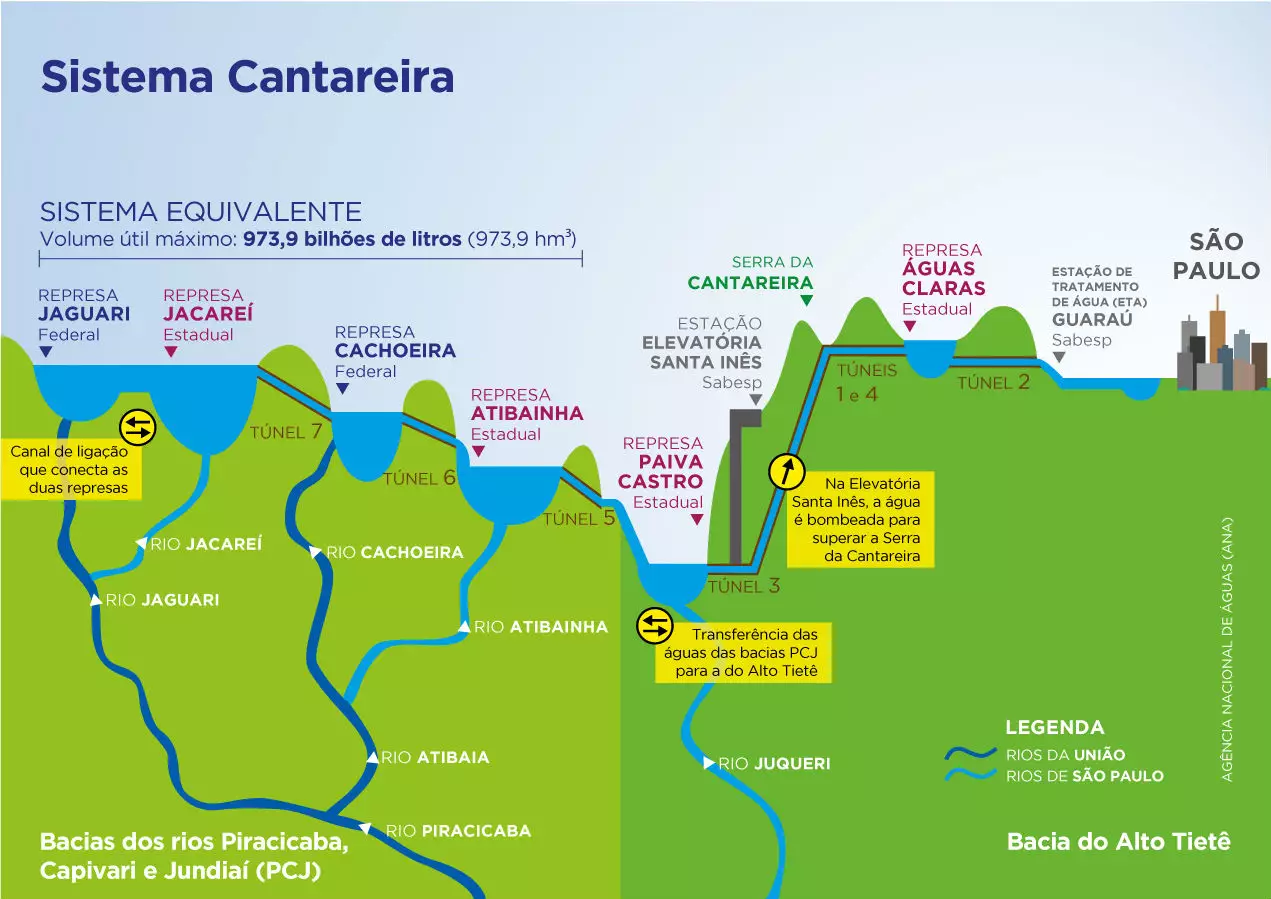
\includegraphics[width=0.8\textwidth,keepaspectratio]{figuras/imagem1.png}
	\fonte{Agência Nacional de Águas e Saneamento Básico (ANA) (2023).}
\end{figure}

A gestão do sistema é de responsabilidade da Agência Nacional de Águas (ANA) e do Departamento de Águas e Energia Elétrica do Estado de São Paulo (DAEE), já a operação do sistema é feita pela Companhia de Saneamento Básico de São Paulo (SABESP), sendo essa a responsável por observar e notificar a necessidade de operações emergenciais em casos excepcionais. Entre as diversas ferramentas de controle utilizadas pela SABESP no Sistema Cantareira, destaca-se a coleta diária de dados da situação operacional — como volumes, vazões e precipitação. Essa atividade representa apenas uma parte do conjunto de ações de monitoramento, mas no escopo deste trabalho, é a principal, uma vez que é o insumo para formar nossa base de dados.  

Os dados coletados permitem acompanhar a situação dos reservatórios, bem como a entrada e saída de água no sistema. Por meio dessas informações, torna-se possível construir análises temporais que evidenciem tendências e padrões de comportamento das variáveis envolvidas. A utilização de séries históricas de volumes, vazões e precipitação possibilita não apenas identificar cenários críticos de forma antecipada, mas também propor medidas de racionalização que contribuam para evitar ou mitigar os efeitos da escassez. Nossa proposta de trabalho concentra-se justamente nesse potencial: oferecer uma ferramenta de apoio às decisões de disponibilização de água pela SABESP, colaborando para reduzir os impactos sociais e econômicos que a má gestão desse recurso essencial pode ocasionar. 

\section{Objetivos Gerais}

\begin{itemize}
    \item Contribuir para a melhoria da gestão dos recursos hídricos no Sistema Cantareira, por meio da análise temporal de dados operacionais, visando antecipar cenários críticos e apoiar decisões de racionalização no abastecimento. 
    \item Utilizar de maneira prática os conhecimentos teóricos aprendidos ao longo do curso e criar uma solução de ciência de dados com arquitetura produtiva. 
\end{itemize}

\subsection{Objetivos Específicos}

\begin{itemize}
    \item Desenvolver uma ferramenta capaz de organizar e analisar séries temporais de variáveis operacionais (volumes e vazões).
    \item Identificar padrões e tendências que permitam prever situações de escassez ou risco no abastecimento.
    \item Propor visualizações e indicadores que facilitem a interpretação dos dados pelos gestores.
\end{itemize}
	
	% 2 - Desenvolvimento
	% ----------------------------------------------------------
\chapter{Fundamentação Teórica}\label{cap:fundamentacao}
% ----------------------------------------------------------
Deve-se inserir texto entre as seções.

\section{Séries Temporais - Conceitos Fundamentais}

\subsection{Definição}

Séries temporais podem ser definidas como a observação de vários registros de uma variável ao longo do tempo, organizada em ordem cronológica \cite{Nielsen}. Segundo \textcite{Hyndman_Athanassopoulos}, diferente de problemas de aprendizado de máquina onde as variáveis são assumidas como independentes e identicamente distribuídas, em séries temporais, há uma dependência entre as variáveis próximas ao longo do tempo, o que exige métodos de análise, modelagem e validação que respeitam a causalidade e estrutura temporal.  

Séries temporais geralmente apresentam componentes estruturados definidos como tendência, sazonalidade, ciclo e resíduos (ou ruído branco), \cite{Hyndman_Athanassopoulos}. Dessa forma, a análise desses dados em série temporal opera sob a premissa de que o valor observado é o resultado da interação simultânea dessas forças. Cada uma dessas componentes atua no comportamento da variável de forma diferente, conforme explicitado a seguir. 

\subsection{Tendência}
A Tendência pode ser definida como o componente que representa o movimento suave e de longo prazo de uma série temporal, refletindo a evolução estrutural do fenômeno observado. Segundo \textcite{Hyndman_Athanassopoulos}, a tendência não necessita ser estritamente linear; ela descreve a direção geral dos dados, ou seja, se é crescente, decrescente ou estável, desconsiderando as flutuações rápidas de curto prazo. \textcite{Morettin_Toloi} complementam que este componente, frequentemente chamado de "movimento secular", pode alterar sua direção ao longo do tempo, revelando pontos de inflexão onde uma série historicamente crescente passa a apresentar um comportamento de declínio. Em dados hidrológicos, por exemplo, isso pode representar a redução gradual do volume armazenado devido a mudanças climáticas ou aumento de demanda ao longo de décadas. 

Do ponto de vista da modelagem em Machine Learning, a tendência é frequentemente tratada como um componente determinístico que pode ser capturado através de engenharia de features. A abordagem mais comum consiste em modelar a tendência em função do tempo, utilizando algoritmos lineares. Matematicamente, uma tendência linear simples pode ser expressa como Tt = B0 + B1t, onde B0 é o intercepto e B1 é a taxa de crescimento. Para tendências simples, utilizando polinômios de grau 1, a regressão linear consegue captar bem o comportamento, porém para tendências mais complexas, a utilização de técnicas de regularização, como Lasso e Ridge, torna-se indispensável ao modelar a tendência através de funções polinomiais de grau superior. 

Conforme destacam James et al. (2021), embora polinômios de grau elevado permitam um ajuste mais flexível aos dados, eles frequentemente sofrem de alta variância, resultando em curvas excessivamente oscilatórias que se superajustam aos dados, causando overfitting do modelo. Esse comportamento é exacerbado nas extremidades da série temporal, um efeito conhecido na análise numérica como Fenômeno de Runge, onde a predição tende a divergir rapidamente. Para minimizar esses riscos, a aplicação de métodos de regularização impõe uma penalidade á magnitude dos coeficientes do modelo, tentando forçar os coeficientes em direção a zero Hastie, Tibshirani e Friedman (2009). Isso garante que a curva de tendência resultante permaneça estável, melhorando a capacidade de generalização do modelo para dados futuros e evitando projeções irrealistas no horizonte de previsão. 

\subsection{Sazonalidade}

A sazonalidade, é um padrão de comportamento que se repete em intervalos de tempo fixos e conhecidos, e que influencia a série temporal de forma regular. Diferentemente de outros movimentos oscilatórios, a principal característica da sazonalidade é a força de sua periodicidade, que pode ser diária, semanal, mensal, anual ou outro intervalo temporal. Segundo Hyndman e Athanasopoulos (2021), a previsibilidade dessa componente da série temporal é alta, justamente por estar relacionada ao calendário e a ciclos naturais bem estabelecidos, o que possibilita sua fácil identificação e modelagem.  

Conforme é evidenciado por Morettin e Toloi (2018), quando se refere a dados hidrológicos, a sazonalidade é frequentemente a manifestação direta de fenômenos climatológicos. As estações do ano estabelecem os regimes pluviométricos, criando períodos de seca e estiagem que podem afetar diretamente o volume dos reservatórios. Essa sazonalidade, de frequência anual, sugere que o comportamento da série temporal, em um determinado mês, por exemplo dezembro, possui alta correlação com o comportamento observado no mesmo mês nos anos anteriores.  

Do ponto de vista de modelagem para aplicações de Machine Learning, a representação matemática da sazonalidade exige estratégias especificas, principalmente na engenharia de features. No contexto de fenômenos naturais como a variação de volume em reservatórios, segundo Hyndman e Athanasopoulos (2021) as séries de Fourier apresentam vantagens significativas sobre o uso de variáveis binárias. Uma vez que dummies tratam a sazonalidade de forma discreta, mudando de nível a cada mês ou período de tempo, os termos de Fourier, composto por funções de seno e cosseno, captam a transição entre períodos de chuva e estiagem por exemplo, e conseguem aproximar melhor a repetição desse padrão hidrológico.   

Ainda sob a ótica de modelagem é importante ressaltar que, modelos lineares como: Regressão Linear, Lasso, Ridge, e Redes Neurais terão melhor desempenho com a modelagem da sazonalidade. Isso se deve ao fato de que um fluxo sazonal, na maioria das vezes é uma junção de diversas sazonalidades primárias, ou seja, possuem movimentações menores e maiores que somadas dão a sazonalidade completa. Os termos de Fourier são ondas de seno e cosseno, somá-las cria uma onda composta melhor, então o modelo linear desenha a curva da sazonalidade naturalmente. Já modelos baseados em árvores, não conseguem fazer esse ajuste, seu princípio está baseado em uma função degrau que criam cortes ortogonais através de condições. Para um modelo de árvores desenhar uma curva sazonal, no formato de onda (senoide), precisaria criar muitas camadas, e resultaria em uma árvore muito profunda, tornando-se menos eficiente que o processo através de modelos lineares.    










	
	% 3 - Seção
	% ----------------------------------------------------------
\chapter{Metodologia}
% ----------------------------------------------------------

\section{Obtenção dos Dados}

Os dados são obtidos via api no site (https://mananciais.sabesp.com.br/api/v4) da SABESP, esses dados são populados diariamente em uma base de consulta pública com informações da   situação nos níveis, vazões, precipitação e demais dados inerentes de cada reservatório individualmente, bem como do Sistema Cantareira Equivalente (SCE), que retrata o sistema como um todo. O SCE, basicamente, é uma agregação dos valores individuais dos reservatórios e suas vazões de tal forma que representem um modelo de sistema um pouco menos complexo. E são esses dados do SCE que foram utilizados neste estudo.

Para as requisições no site da SABESP enviamos parâmetros para designar o que queremos extrair, são eles: Data de Início; Data Fim; Número que indica o reservatório ou SCE (em nosso estudo, utilizamos para o SCE). O retorno dessa requisição é um json com todas as informações sobre o SCE para a data determinada que estamos fazendo a coleta.

Apesar dos dados serem atualizados diariamente, devido a variação diária ser muito baixa no volume (pelo próprio conceito físico), optamos por fazer extrações semanais dos dados. A Tabela \ref{tab:dados_cantareira} mostra o formato final dos dados que obtivemos.

\begin{table}[H]
	\centering
	\caption{Exemplo de dados do Sistema Cantareira Equivalente (SCE).}
	\label{tab:dados_cantareira}
	\small
	\resizebox{\textwidth}{!}{
	\begin{tabular}{|c|c|c|c|c|c|c|}
		\hline
		\textbf{Data} & \textbf{Chuva} & \textbf{Volume Útil} & \textbf{Volume Útil} & \textbf{Volume Total} & \textbf{Vazão} & \textbf{Vazão} \\
		& \textbf{(mm)} & \textbf{Armazenado (\%)} & \textbf{Armazenado (hm³)} & \textbf{Armazenado (hm³)} & \textbf{Jusante (m³/s)} & \textbf{Natural (m³/s)} \\
		\hline
		01/01/2000 & 30,900 & 47,11 & 365,51 & 1072,05 & 10,16 & 70,89 \\
		\hline
		02/01/2000 & 29,100 & 47,78 & 370,65 & 1077,19 & 10,18 & 94,86 \\
		\hline
		03/01/2000 & 35,175 & 48,59 & 377,00 & 1083,55 & 7,29 & 108,21 \\
		\hline
		04/01/2000 & 18,725 & 50,00 & 387,88 & 1094,43 & 6,34 & 162,94 \\
		\hline
		05/01/2000 & 25,900 & 51,95 & 403,00 & 1109,55 & 6,33 & 211,60 \\
		\hline
	\end{tabular}
	}
	\fonte{Elaborado pelos autores com base em dados da SABESP (2025).}
\end{table}

\section{Análise das Variáveis} 

\subsection{Variável Alvo - Volume Útil(\%)}

O objetivo será através das previsões notificar se o volume útil atingirá essa marca no horizonte projetado. Entendendo melhor o que cada variável representa podemos começar a destrinchar a análise sobre cada uma delas para identificar e entender comportamentos que servirão de base para nossa modelagem mais adiante. Na Figura \ref{fig:Fig_3} a seguir, é possível visualizar o gráfico de linha da série temporal de todo período de dados coletado da nossa variável alvo. 

\begin{figure}[H]
	\centering
	\caption{Volume Útil(\%) do Sistema Cantareira entre 2000 e 2025.}
	\label{fig:Fig_3}
	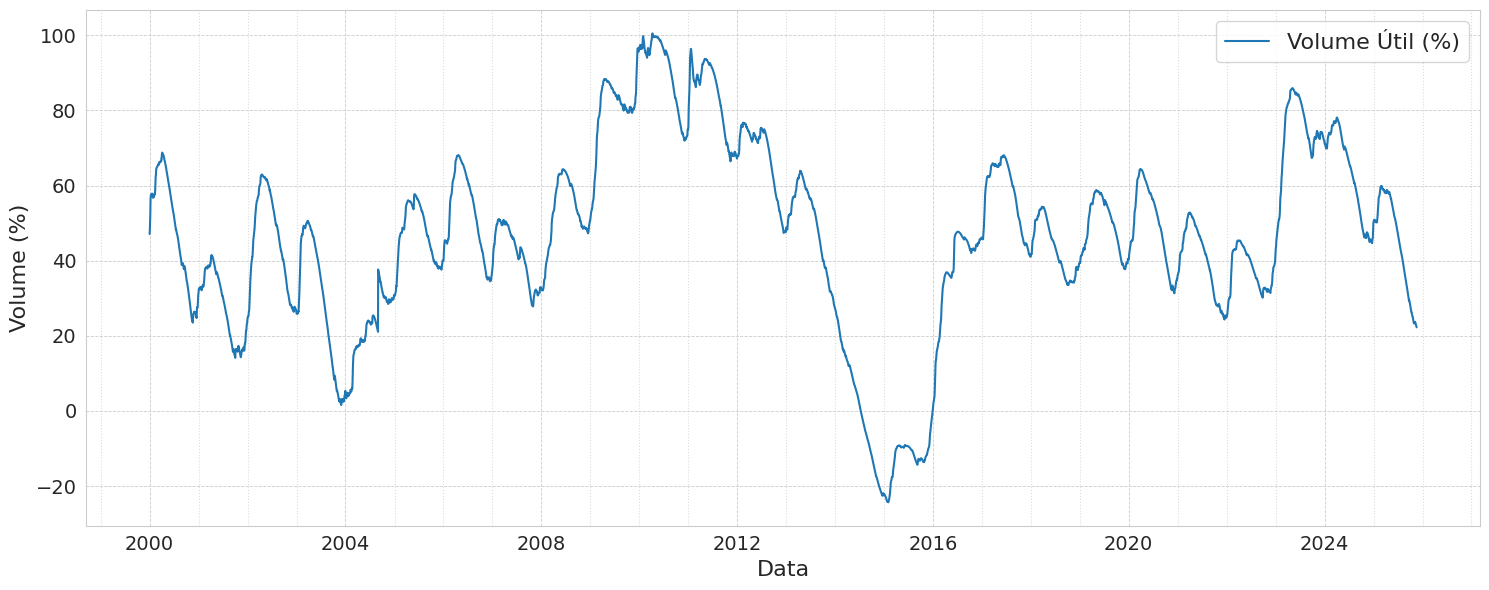
\includegraphics[width=0.9\textwidth,keepaspectratio]{figuras/imagem3.png}
	\fonte{Elaborado pelos autores com base em dados da SABESP (2025).}
\end{figure}

Observando o gráfico da Figura x, é possível identificar alguns comportamentos nos dados, como por exemplo o aumento e diminuição no volume em virtude dos períodos de chuva e seca ao longo das estações do ano. Nota-se que não há variações bruscas no volume, o aumento e diminuição ocorre de forma gradativa, em valores predominantemente nas faixas normais e de atenção. No entanto, em períodos excepcionais como a crise hídrica entre 2014 e 2015, é possível ver que o comportamento da variável permanece por período prolongado em níveis de alerta, restrição e excepcional, episódios que evidenciam condições hidrológicas adversas persistentes, distintas do padrão sazonal observado na maior parte do período analisado. Na Figura \ref{fig:Fig_4} a seguir, podemos visualizar como se comporta essa distribuição dos valores ao longo do ano.  

É curioso observar que, conforme será mostrado na análise de variáveis exógenas, o período chuvoso ocorre entre outubro e março, porém os meses de cheia no reservatório ocorre fora desse período, o que mostra que a chuva pode não ter ação imediata sobre o volume do reservatório, mas um efeito a médio longo prazo, influenciando primeiro nos rios e mananciais que alimentam o reservatório e contribuindo para aumentar a vazão natural por exemplo, que ai sim de fato espera-se que influencie mais no volume útil armazenado.  

\begin{figure}[H]
	\centering
	\caption{Distribuição anual do Volume Útil(\%) do Sistema Cantareira entre 2000 e 2025.}
	\label{fig:Fig_4}
	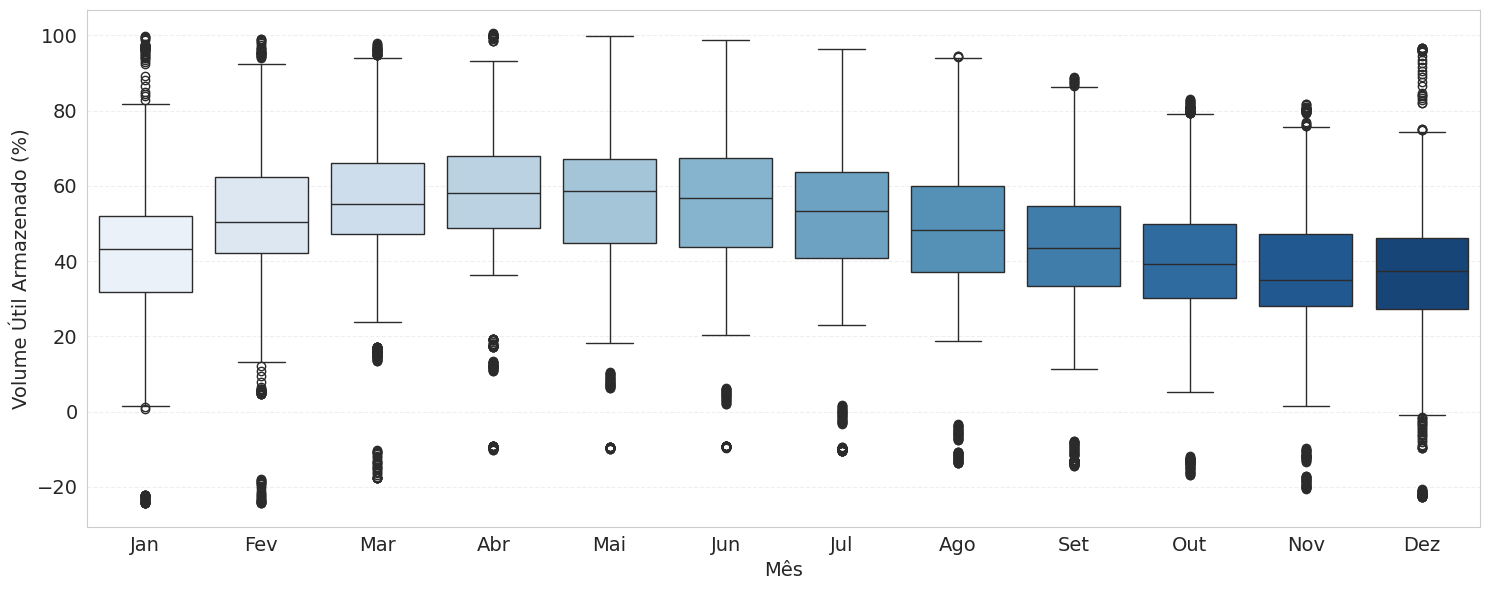
\includegraphics[width=0.9\textwidth,keepaspectratio]{figuras/imagem4.png}
	\fonte{Elaborado pelos autores com base em dados da SABESP (2025).}
\end{figure}

Parte importante da análise de dados em série temporal, é a visualização das componentes da mesma, separadamente. Na \autoref{fig:Fig_5} a seguir é possível visualizar as componentes de tendência, sazonalidade e resíduos. A tendência mostra o comportamento de movimento da variável medida, se ela está aumentando ou diminuindo ao longo do tempo, a componente de sazonalidade, mostra com que frequência o padrão de comportamento da variável se repete ao longo da série, num período de tempo, neste caso podemos visualizar uma sazonalidade anual pois a curva se repete anualmente no gráfico, e por fim a componente de resíduos que é o que sobra depois que se remove as componentes anteriores, é a parte com comportamento irregular da série. 

\begin{figure}[H]
	\centering
	\caption{Decomposição da série temporal do Volume Útil(\%) do Sistema Cantareira entre 2000 e 2025.}
	\label{fig:Fig_5}
	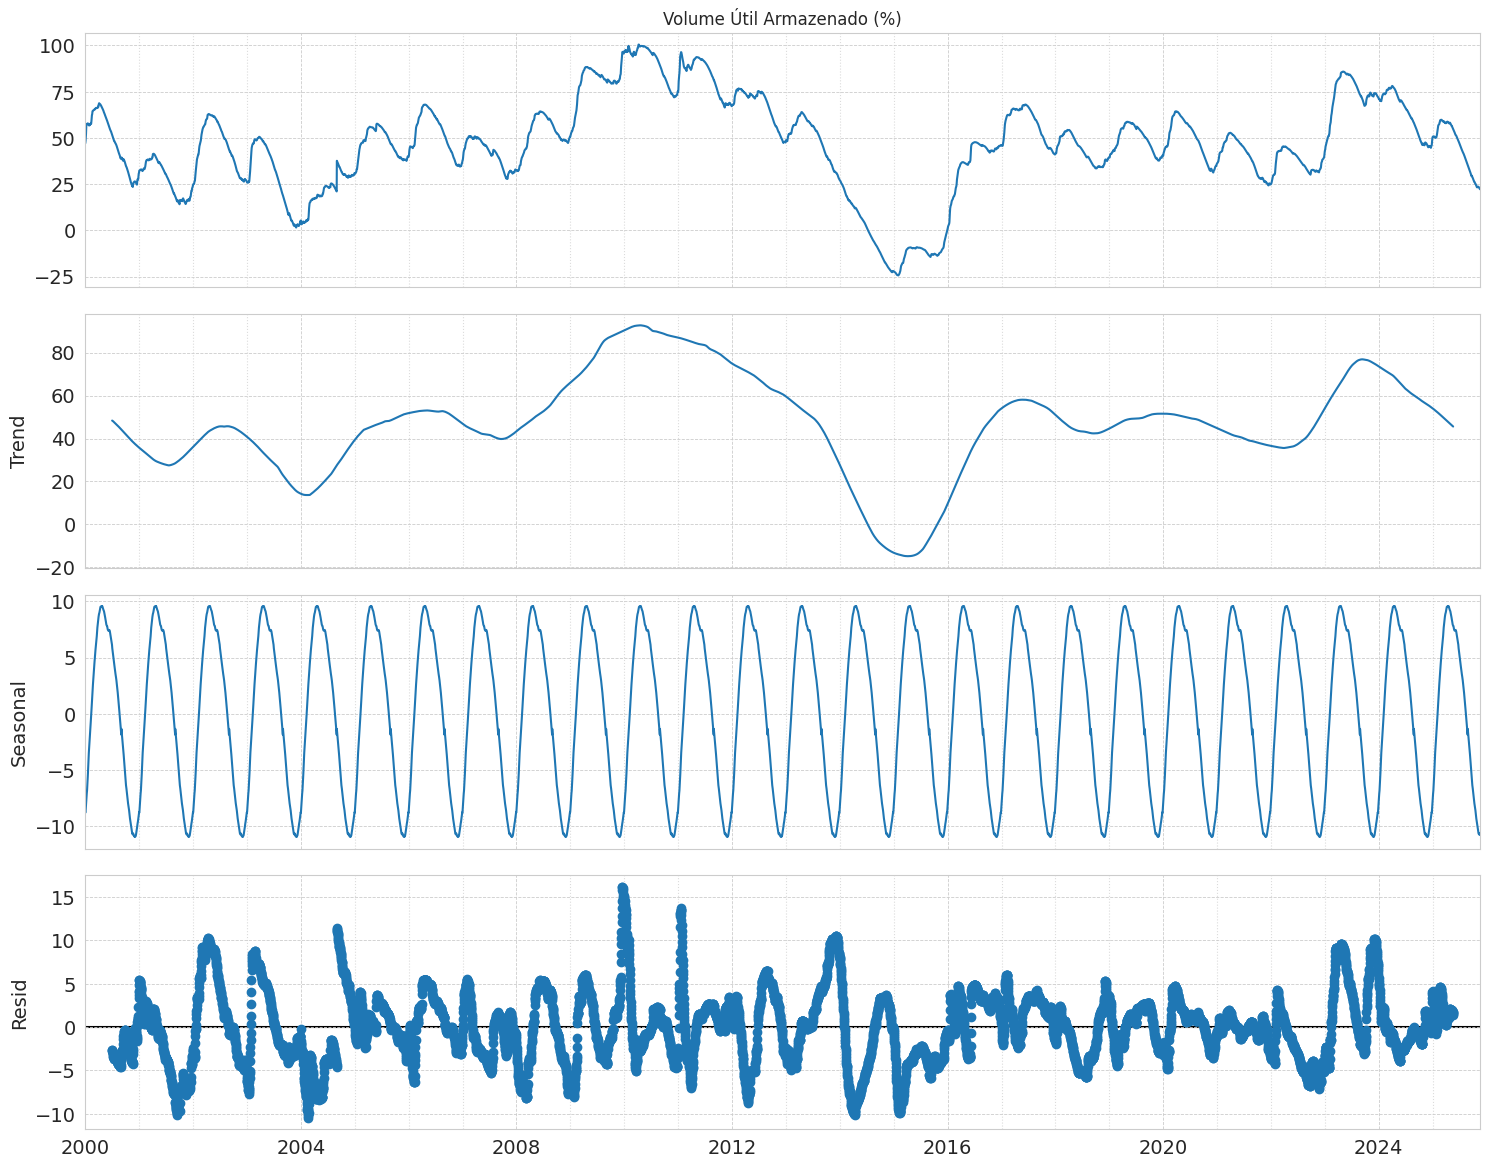
\includegraphics[width=0.9\textwidth,keepaspectratio]{figuras/imagem5.png}
	\fonte{Elaborado pelos autores com base em dados da SABESP (2025).}
\end{figure}

Outra análise realizada sobre sazonalidade a sazonalidade da variável alvo, foi o periodograma, que por sua vez, tem o objetivo de identificar ciclos repetitivos nos dados. A \autoref{fig:Fig_6} a seguir, confirma que existe de fato uma periodicidade anual nos dados como havia sido interpretado na decomposição da série temporal na \autoref{fig:Fig_5}, e além disso, podemos observar que há outras periodicidades como tetra ou octo anual, que podem estar relacionados a eventos climáticos que influenciaram na chegada de água do reservatório causando períodos de extrema seca ou picos de cheia dos reservatórios. Por exemplo no gráfico da \autoref{fig:Fig_3}, é possível visualizar a ocorrência de valores extremos nos dados numa frequência bem maior do que anual.  

\begin{figure}[H]
	\centering
	\caption{Periodograma do Volume Útil(\%) do Sistema Cantareira entre 2000 e 2025.}
	\label{fig:Fig_6}
	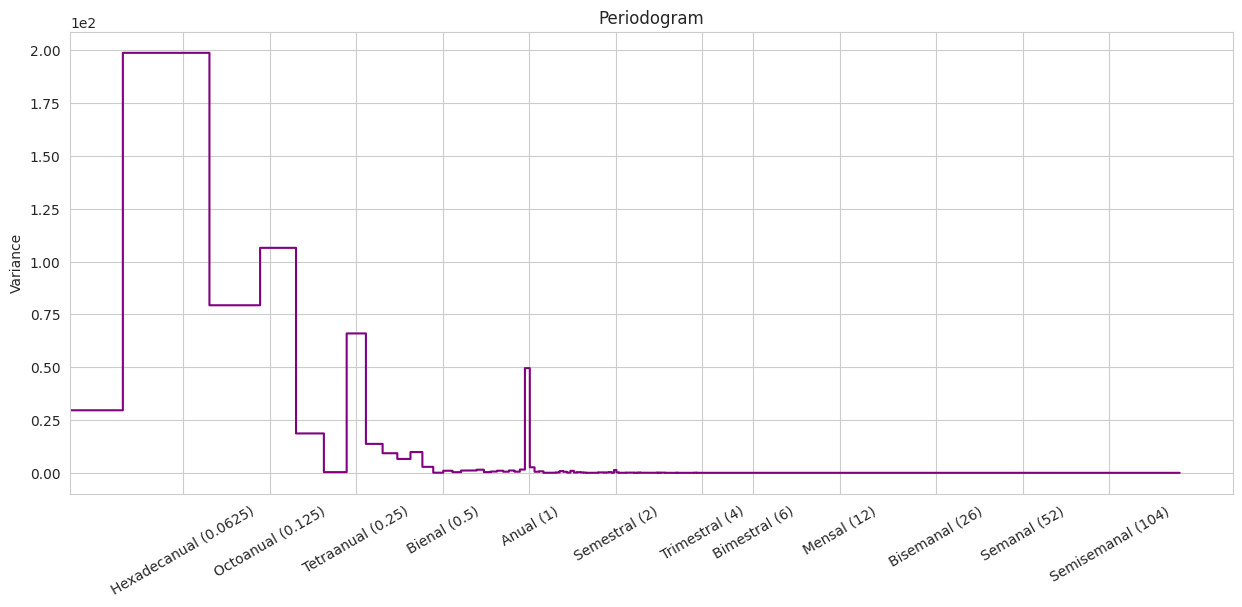
\includegraphics[width=0.9\textwidth,keepaspectratio]{figuras/imagem6.png}
	\fonte{Elaborado pelos autores com base em dados da SABESP (2025).}
\end{figure}

Outro aspecto fundamental de uma série temporal que foi analisado, é a relação da variável com os seus valores anteriores, visto que a modelagem de uma série temporal tem, entre outros objetivos, aprender comportamentos com os dados do passado, para prever cenários futuros \cite{Nielsen}. A \autoref{fig:Fig_7} a seguir, mostra a autocorrelação e a autocorrelação parcial da variável alvo, a autocorrelação nos mostra que a variável alvo possui uma inércia alta, ou seja, varia lentamente, no dia 1 a autocorrelação é 1, e no dia 60 ainda está muito próximo de 1. E com a autocorrelação parcial, podemos concluir que o volume do dia anterior é praticamente o volume de hoje, ou seja, o lag 1 pode ser uma ótima variável preditora já que a PACF é 1. Entretando pode-se observar que o mesmo já não vale para o lag 2 em diante, pois a PACF cai abruptamente.  

\begin{figure}[H]
	\centering
	\caption{Gráfico de Autocorrelação e Autocorrelação Parcial do Volume Útil(\%) do Sistema Cantareira entre 2000 e 2025.}
	\label{fig:Fig_7}
	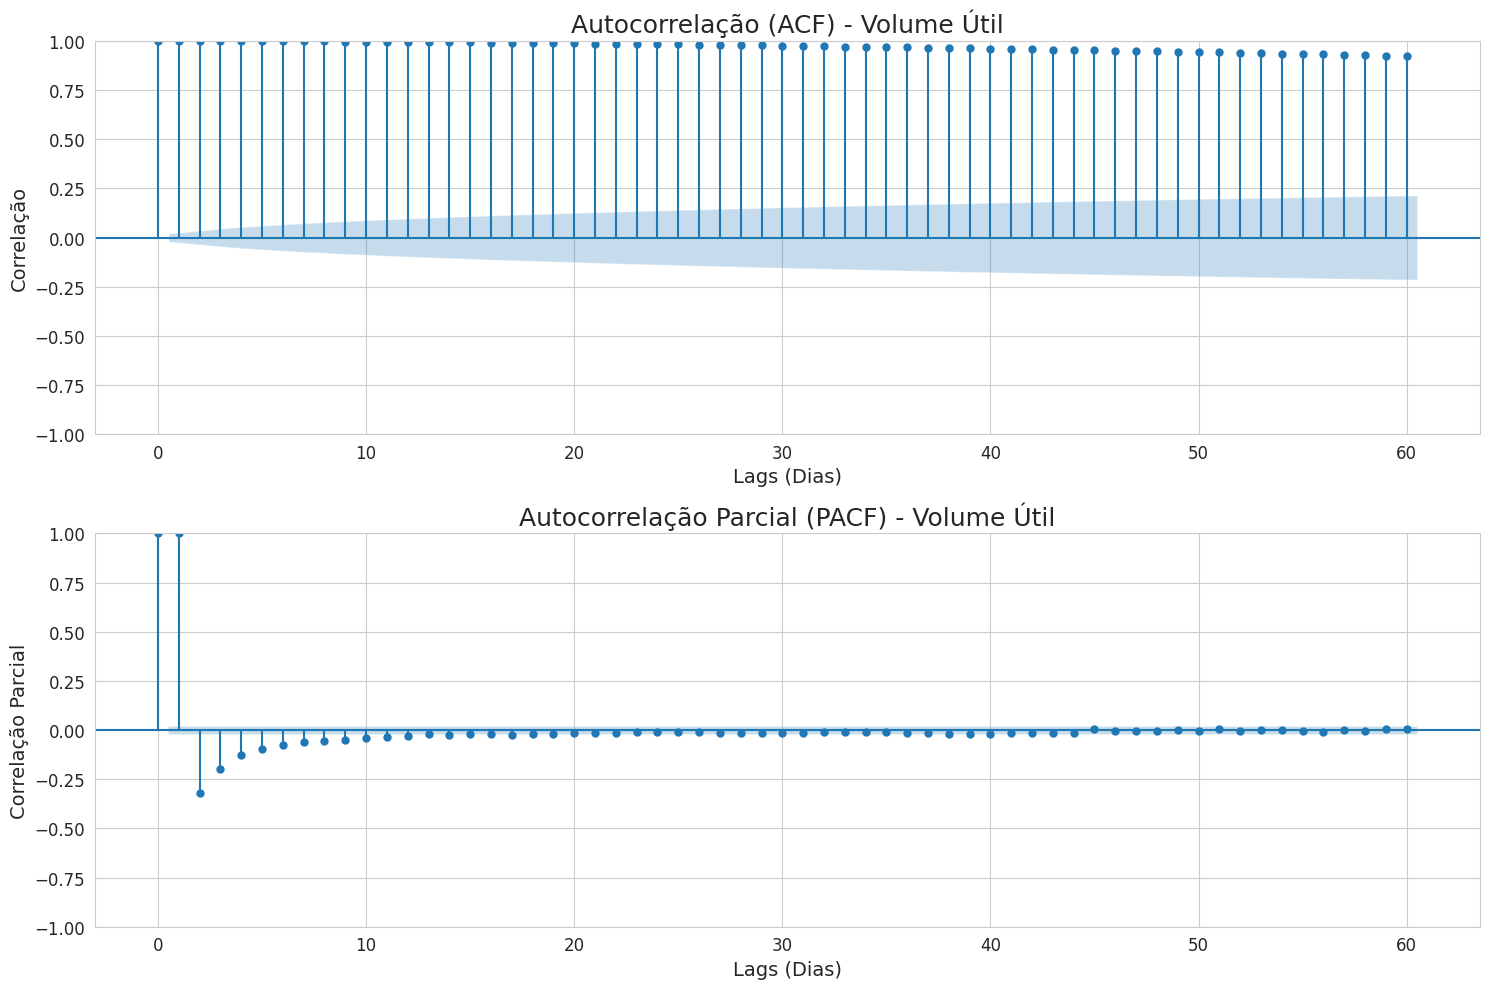
\includegraphics[width=0.9\textwidth,keepaspectratio]{figuras/imagem7.png}
	\fonte{Elaborado pelos autores com base em dados da SABESP (2025).}
\end{figure}

\subsection{Variáveis Exógenas}

Variáveis exóginas são variáveis externas que impactam no valor de uma série temporal, essas variáveis podem ser independentes do tempo, como por exemplo, ao prever vendas, podemos usar uma variável que diz se houve campanha de marketing ou não em um determinado período; ou elas podem ser dependentes do tempo, como por exemplo, considerar o número de vendas de pão de queijo para prever o número de vendas de café. 

São diversos os fatores que podem influenciar no aumento ou diminuição do volume útil do reservatório, como fatores muito influentes podemos citar: a precipitação, a vazão natural que representa o volume de água que chega nos reservatórios, a vazão jusante que é o volume de água que sai dos reservatórios, e até outros fatores como: evaporação, consumo, etc. Para este estudo, obteve-se melhores resultados nos modelos ao utilizar as variáveis exógenas de vazão natural e vazão jusante, como variáveis preditoras elas auxiliaram o modelo a realizar uma previsão do volume útil mais próxima do real.  

Realizamos alguns testes para verificar se havia influência direta da variável na predição do volume, dentre eles, a criação de um modelo com a tendência e sazonalidade do volume e o valor real da candidata a variável exógina (vazão natural, vazão jusante e chuva), nestes testes, observamos que a mais considerável para a previsão do volume é a vazão natural, seguida da vazão jusante e por fim, com menos efeito, a chuva. Além disso, testamos modelos combinando ambas as variáveis exóginas para avaliar quais eram mais influentes no aprendizado do modelo, neste caso, a influência da chuva se faz menos gritante, porque a parcela que influenciaria, é capturada pela vazão natural.  

Ao observar que a variável de vazão natural e jusante possuíam influência forte, decidimos por utilizar elas no modelo, entretanto, caímos em um problema de prever  o comportamento dessas variáveis, uma vez que são variáveis dependentes do tempo e essas previsões necessitam ser bem assertivas (comportamentais) para influenciar positivamente o modelo. Erros altos nessas variáveis levarão a previsões muito ruins no volume, uma vez que são variáveis determinantes.  Neste estudo optou-se por construir um modelo que realiza a previsão das variáveis de vazão para posteriormente usá-la para construir novas variáveis preditoras para os modelos de previsão de volume, isso será detalhado na seção que tratará da modelagem.  

\subsubsection{Vazão Natural e Vazão Jusante}

Conforme já definido anteriormente, a vazão natural ou montante representa a porção que chega no reservatório, ela está intimamente ligada a ocorrência de precipitação dentro da bacia hidrográfica, que vai alimentar rios, mananciais, lençóis freáticos e escoar para as reservas. Na \autoref{fig:Fig_8} a seguir, temos o gráfico da variável ao longo do período analisado, e podemos observar que assim como a varável de volume, esta apresenta um comportamento que parece se repetir ao longo do tempo. Isso pode estar relacionado a forte relação que essa variável pode ter com o ciclo hidrológico e as estações chuvosas.  

\begin{figure}[H]
	\centering
	\caption{Histórico da Vazão Natural do Sistema Cantareira entre 2000 e 2025.}
	\label{fig:Fig_8}
	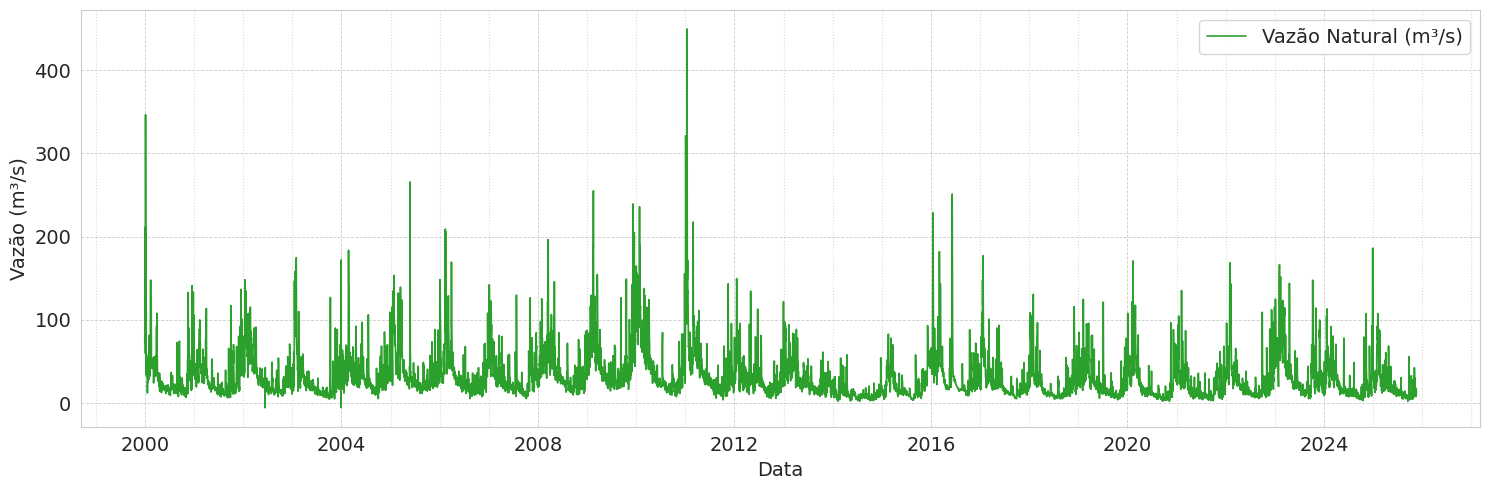
\includegraphics[width=0.9\textwidth,keepaspectratio]{figuras/imagem8.png}
	\fonte{Elaborado pelos autores com base em dados da SABESP (2025).}
\end{figure}

No gráfico da \autoref{fig:Fig_8} acima, ainda, nota-se que ocorrem muitos picos de vazão, mas é possível perceber um comportamento de aumento e diminuição da vazão ao longo do ano, isso é esperado uma vez que a vazão natural conforme mencionado, depende do ciclo hidrológico e consequentemente depende bastante da precipitação. Desta forma é possível relacionar o aumento ou diminuição da vazão com os períodos de chuva e estiagem. No boxplot da \autoref{fig:Fig_9} a seguir, é possível ver que as vazões são maiores no período chuvoso que ocorre entre outubro e março, informação que pode ser confirmada no gráfico da \autoref{fig:Fig_10} logo em seguida, onde os meses com maior volume de precipitação de acordo com os dados do Sistema Equivalente Cantareira, também foram entre outubro e março.  

\begin{figure}[H]
	\centering
	\caption{Distribuição anual da Vazão Natural do Sistema Cantareira entre 2000 e 2025.}
	\label{fig:Fig_9}
	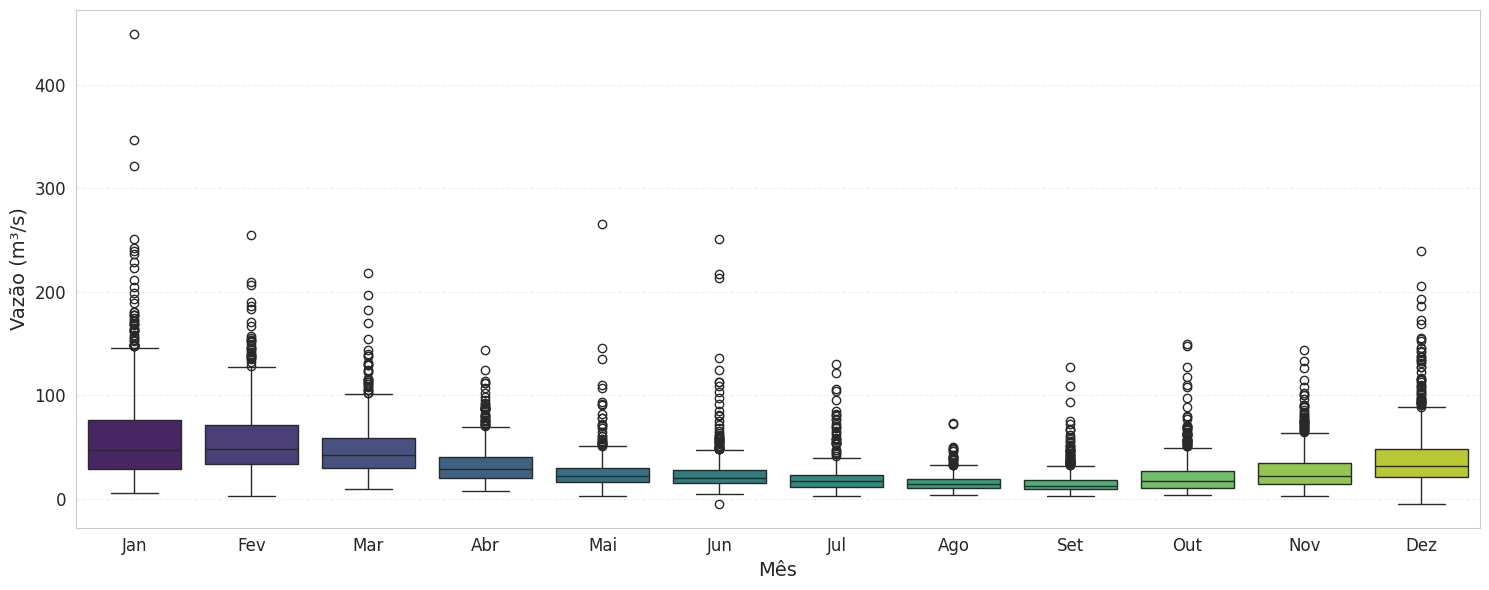
\includegraphics[width=0.9\textwidth,keepaspectratio]{figuras/imagem9.png}
	\fonte{Elaborado pelos autores com base em dados da SABESP (2025).}
\end{figure}

\begin{figure}[H]
	\centering
	\caption{Distribuição anual da Chuva (mm)do Sistema Cantareira entre 2000 e 2025.}
	\label{fig:Fig_10}
	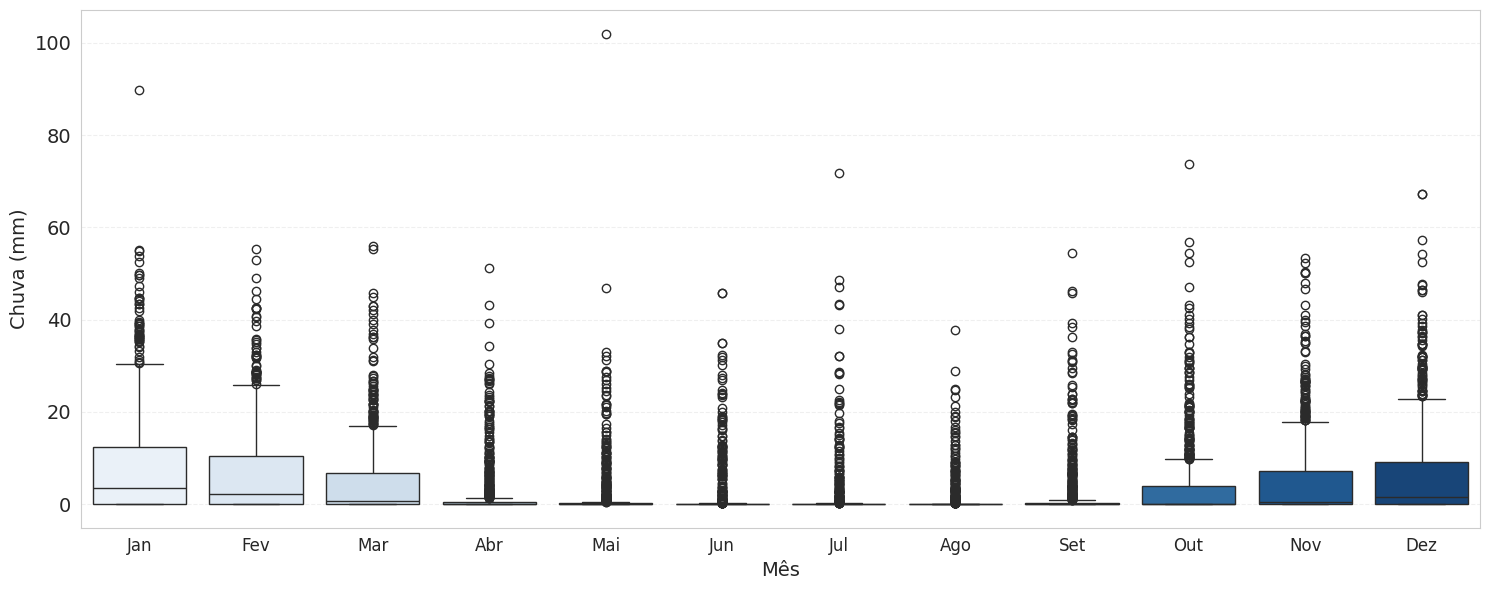
\includegraphics[width=0.9\textwidth,keepaspectratio]{figuras/imagem10.png}
	\fonte{Elaborado pelos autores com base em dados da SABESP (2025).}
\end{figure}

Com isso, espera-se que a variável exógena de vazão natural auxilie os modelos a entenderem o comportamento do volume útil, visto que seu comportamento acompanha períodos de cheia e estiagem, então espera-se que conforme esta variável varie, mostre ao modelo como o volume deve variar. Entretanto, um dos maiores desafios na utilização de variáveis exógenas, principalmente que acontecem em decorrência de fatores naturais, e variam muito, é como prever seus valores para o futuro, garantindo a qualidade dos dados que vamos entregar para o modelo de previsão de volume, os métodos utilizados neste estudo para modelagem e obtenção dessa variável serão discutidos nos próximos capítulos.  

Por sua vez, a vazão jusante, representa o oposto da vazão natural, ela é a saída de água dos reservatórios, seja para abastecimento ou alimentar outros reservatórios e represas. A vazão jusante não é um evento natural como a precipitação e a vazão natural, ela depende da demanda de utilização da água e pode ser controlada conforme gestão da operadora do sistema, a SABESP. Mas está diretamente relacionada ao volume útil dos reservatórios, visto que picos constantes de retirada de água dos mesmos, poderiam ocasionar uma diminuição anormal do volume armazenado, bem como a ocorrência de valores negativos de entrada liquida no reservatório, ou seja, a vazão jusante maior do que a vazão natural, o que pode ocorrer principalmente nos períodos em que se observa vazões naturais muito baixas. Neste sentido, há um entendimento físico de que a SABESP tem liberdade para aumentar ou reduzir essa vazão e, utiliza deste artifício para garantir abastecimento da população de forma que não atinjamos o volume morto ou o reservatório passe a perder perenidade 

No gráfico da \autoref{fig:Fig_11} a seguir, pode-se observar a distribuição da vazão jusante comparada a vazão montante ao longo do período analisado, nota-se que os valores são bem menores do que os observados para vazão natural, salvo alguns picos observados em pontos específicos do gráfico. Um aspecto interessante do comportamento dessa variável, é que seu valor varia pouco comparado a variação que acontece nas variáveis que foram analisadas anteriormente. Ainda assim, é possível perceber um aumento nos valores de saída quando se aproxima do final do ano, seguido de uma queda nos meses que antecede o verão, que pode estar relacionado ao racionamento no fornecimento, que geralmente ocorre próximo do verão para controle dos gastos com água, e que coincide com épocas em que o volume do reservatório geralmente está baixo devido ao período de seca que ocorre até setembro, o que pode justificar tais ações por parte da SABESP.  

\begin{figure}[H]
	\centering
	\caption{Histórico da Vazão Jusante do Sistema Cantareira entre 2000 e 2025.}
	\label{fig:Fig_11}
	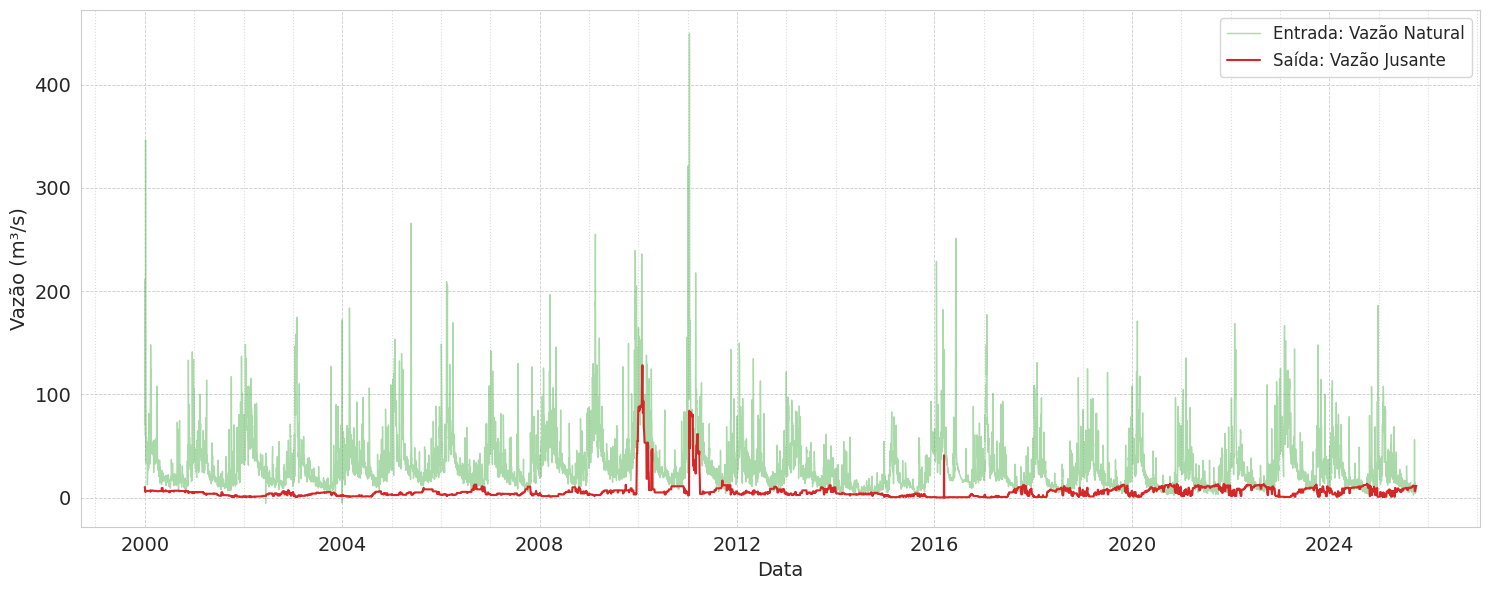
\includegraphics[width=0.9\textwidth,keepaspectratio]{figuras/imagem11.png}
	\fonte{Elaborado pelos autores com base em dados da SABESP (2025).}
\end{figure}

\begin{figure}[H]
	\centering
	\caption{Distribuição anual da Vazão Jusante do Sistema Cantareira entre 2000 e 2025.}
	\label{fig:Fig_12}
	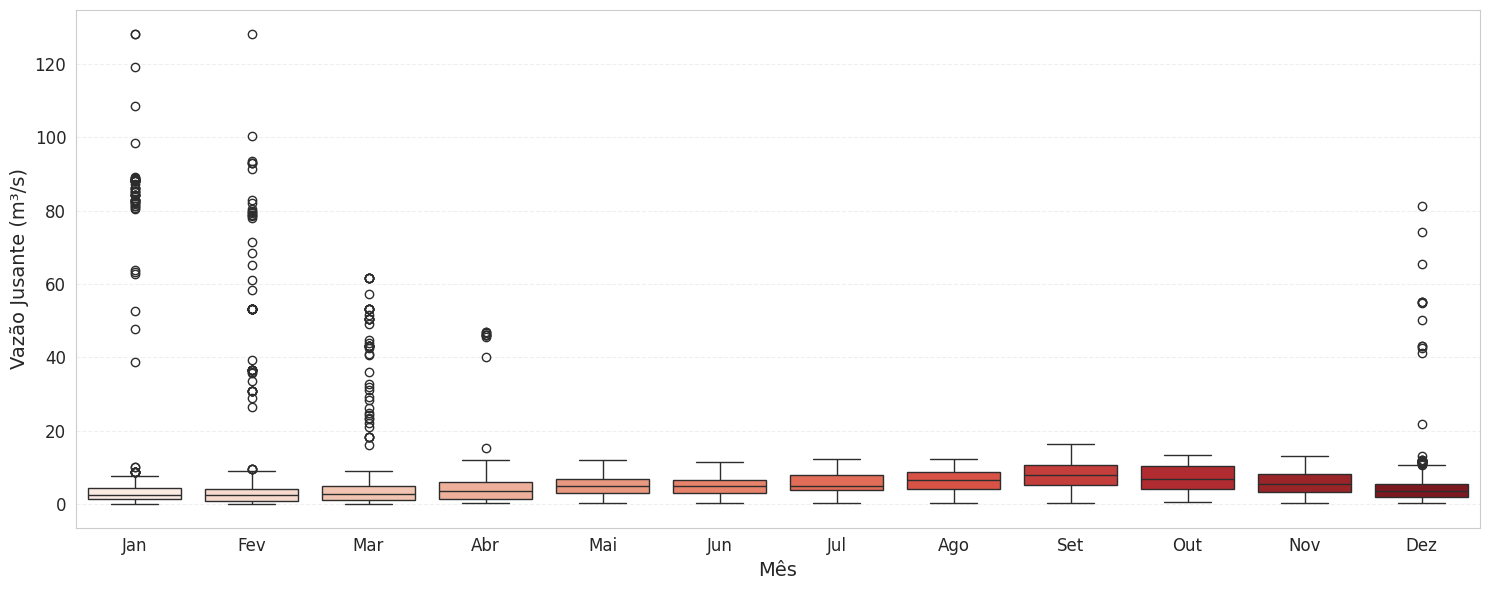
\includegraphics[width=0.9\textwidth,keepaspectratio]{figuras/imagem12.png}
	\fonte{Elaborado pelos autores com base em dados da SABESP (2025).}
\end{figure}

Uma vez que teremos que modelar as vazões natural e jusante por meio de series temporais, é relevante avaliar alguns gráficos que nos auxiliam a realizar essa modelagem, são eles: o periodograma que nos ajuda a identificar sazonalidade e estimar valores para os ciclos das funções seno e cosseno da série de Fourier; A autocorrelação (ACF) que mede a correlação dos lags da variável com o ela mesma, auxiliando também na identificação de tendência e sazonalidade; A autocorrelação parcial (PACF) que mede a influência de um lag na variável, de forma a excluir efeitos de lags intermediários. Esses gráficos nos ajudam a entender quantos Lags de variável utilizar, como o polinômio de tendência pode ser bem modelado e achar valores para a sazonaldiade.  

As figuras \autoref{fig:Fig_13} e \autoref{fig:Fig_14} mostram o periodograma da vazão jusante e da vazão natural, respectivamente.

\begin{figure}[H]
	\centering
	\caption{Periodograma da Vazão Jusante do Sistema Cantareira entre 2000 e 2025.}
	\label{fig:Fig_13}
	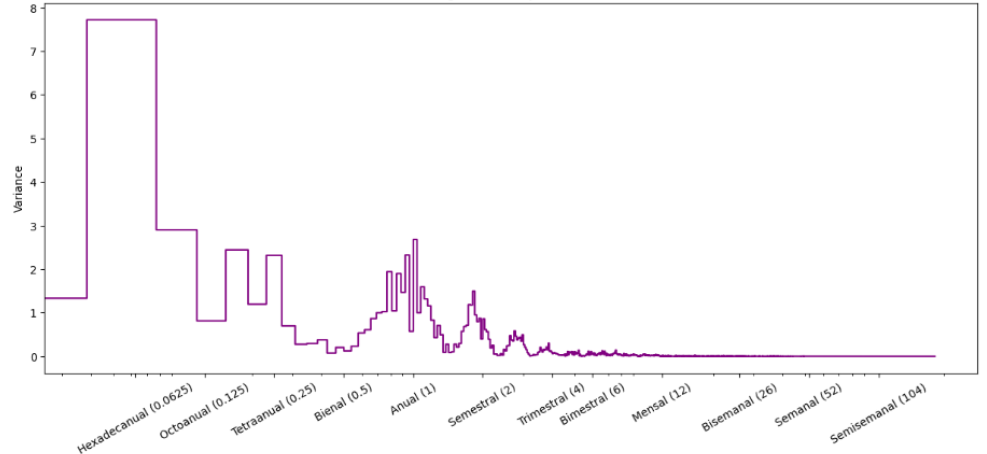
\includegraphics[width=0.9\textwidth,keepaspectratio]{figuras/imagem13.png}
	\fonte{Elaborado pelos autores com base em dados da SABESP (2025).}
\end{figure}

\begin{figure}[H]
	\centering
	\caption{Periodograma da Vazão Natural do Sistema Cantareira entre 2000 e 2025.}
	\label{fig:Fig_14}
	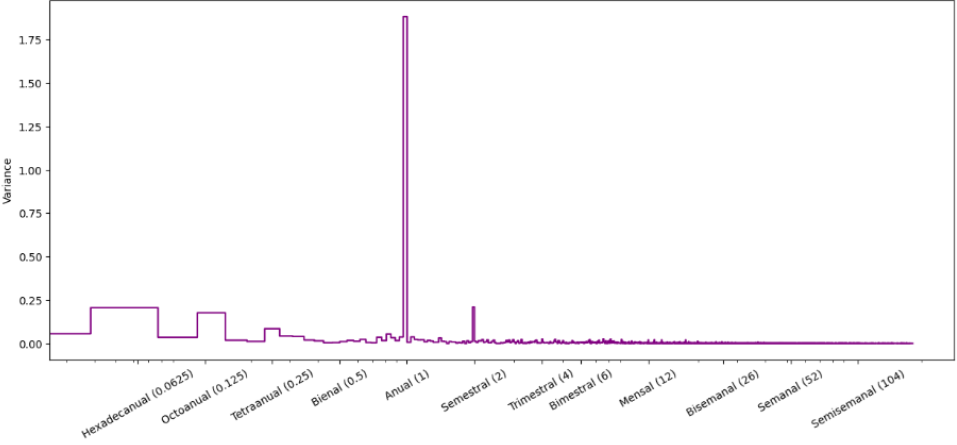
\includegraphics[width=0.9\textwidth,keepaspectratio]{figuras/imagem14.png}
	\fonte{Elaborado pelos autores com base em dados da SABESP (2025).}
\end{figure}

Para a vazão jusante, podemos ver que ele é bem mais irregular, uma vez que não é uma variável espontânea e varia com ação humana, mas, podemos considerar como frequência anual uma boa estimativa.  Já para a vazão natural, fica mais claro o pico na frequência anual, apesar de ser um pico com largura curta, para períodos maiores parece haver ainda frequências boas e menores, parece ser apenas ruído, então frequência anual também parece uma boa estimativa. 

As figuras \autoref{fig:Fig_13}, \autoref{fig:Fig_13}, \autoref{fig:Fig_13} e \autoref{fig:Fig_14} a seguir, apresentam as autocorrelações e autocorrelações parciais da vazão natural, bem como as autocorrelações e autocorrelações parciais de seus resíduos (vazão natural sem tendencia e sazonaldiade). 

\begin{figure}[H]
	\centering
	\caption{Gráfico da Autocorrelação Parcial do Residuo da Vazão Natural após remover tendência e sazonalidade.}
	\label{fig:Fig_15}
	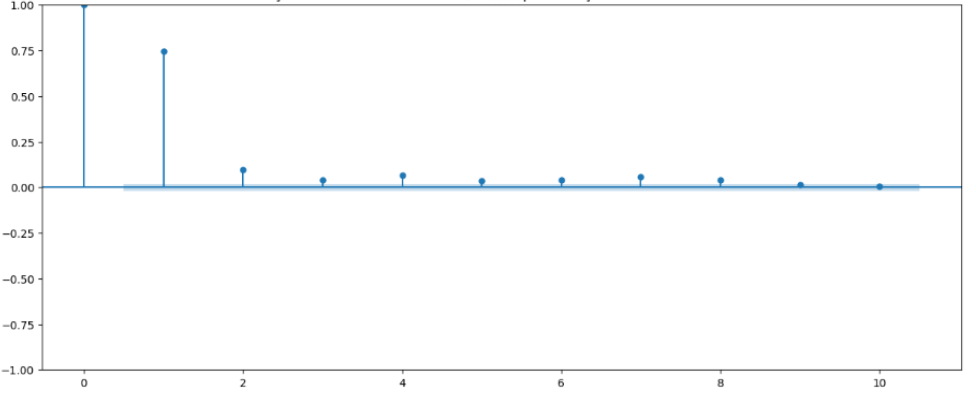
\includegraphics[width=0.9\textwidth,keepaspectratio]{figuras/imagem15.png}
	\fonte{Elaborado pelos autores com base em dados da SABESP (2025).}
\end{figure}

\begin{figure}[H]
	\centering
	\caption{Gráfico da Autocorrelação Parcial do Residuo da Vazão Natural.}
	\label{fig:Fig_16}
	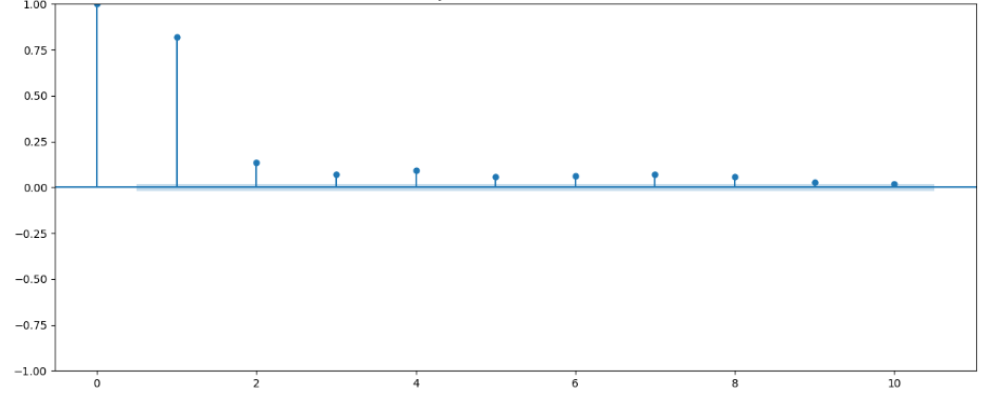
\includegraphics[width=0.9\textwidth,keepaspectratio]{figuras/imagem16.png}
	\fonte{Elaborado pelos autores com base em dados da SABESP (2025).}
\end{figure}

\begin{figure}[H]
	\centering
	\caption{Gráfico da Autocorrelação do Residuo da Vazão Natural após remover tendência e sazonalidade.}
	\label{fig:Fig_17}
	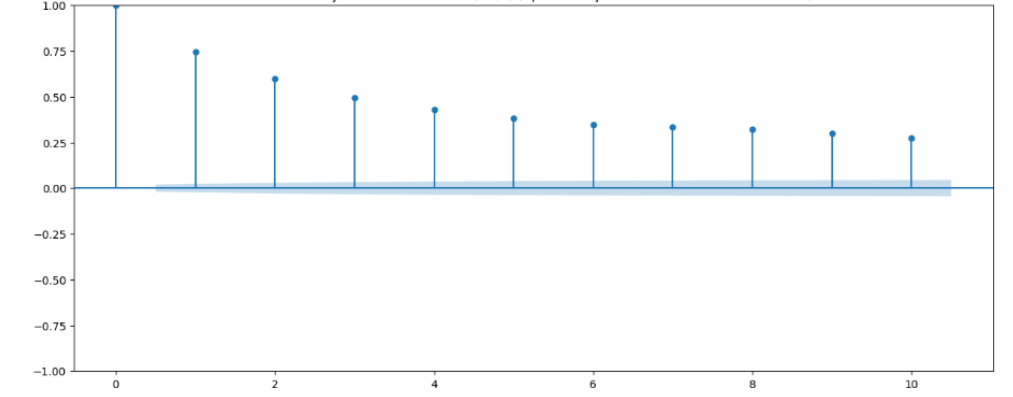
\includegraphics[width=0.9\textwidth,keepaspectratio]{figuras/imagem17.png}
	\fonte{Elaborado pelos autores com base em dados da SABESP (2025).}
\end{figure}

\begin{figure}[H]
	\centering
	\caption{Gráfico da Autocorrelação do Residuo da Vazão Natural.}
	\label{fig:Fig_18}
	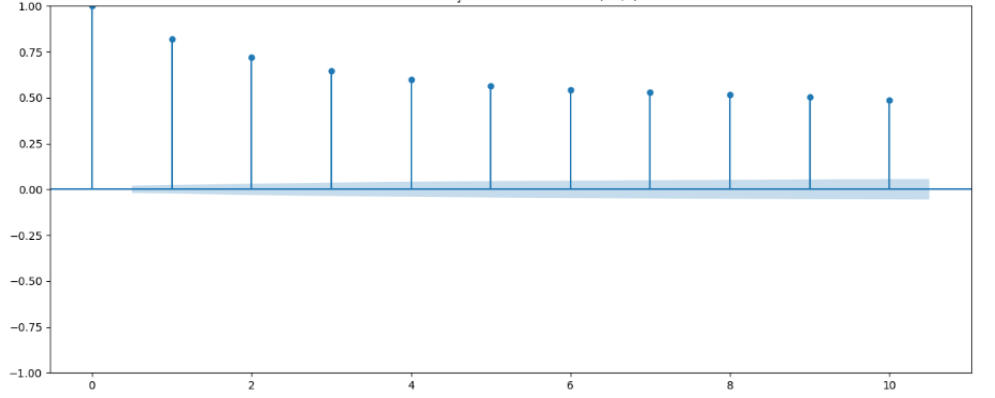
\includegraphics[width=0.9\textwidth,keepaspectratio]{figuras/imagem18.png}
	\fonte{Elaborado pelos autores com base em dados da SABESP (2025).}
\end{figure}

Como podemos ver, há uma forte correlação da variável (e de seu resíduo) com o lag com defasagem de 1, isto ocorre porque as variações no reservatório são um pouco lentas, além disso, pelos gráficos podemos ver que a influência parcial dos outros lags cai muito, apesar da autocorrelação total ser alta, isto se deve ao fato de que na autocorrelação total, a influência do lag 1 é propagada para os outros lags. Desta forma, seria interessante utilziar lag1 ou lag2 como variáveis para modelar a vazão natural. 

As figuras \autoref{fig:Fig_13}, \autoref{fig:Fig_13}, \autoref{fig:Fig_13} e \autoref{fig:Fig_14} a seguir, apresentam as autocorrelações e autocorrelações parciais da vazão jusante, bem como as autocorrelações e autocorrelações parciais de seus resíduos (vazão jusante sem tendencia e sazonaldiade). 

\begin{figure}[H]
	\centering
	\caption{Gráfico da Autocorrelação Parcial do Residuo da Vazão Jusante após remover tendência e sazonalidade.}
	\label{fig:Fig_19}
	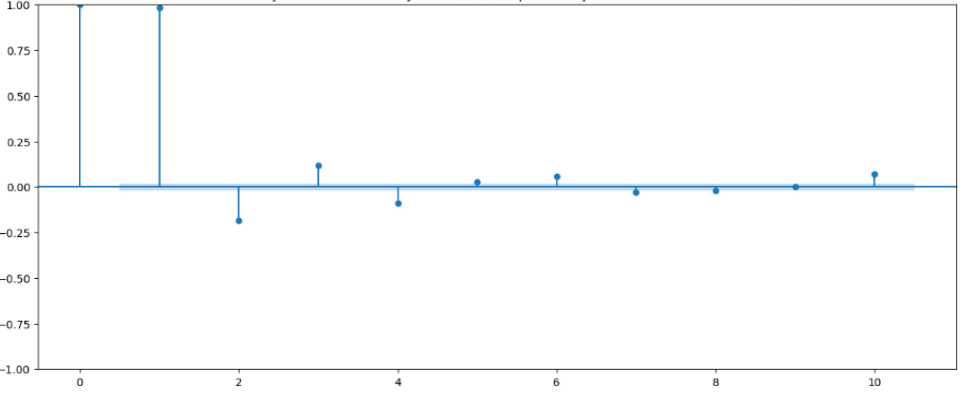
\includegraphics[width=0.9\textwidth,keepaspectratio]{figuras/imagem19.png}
	\fonte{Elaborado pelos autores com base em dados da SABESP (2025).}
\end{figure}

\begin{figure}[H]
	\centering
	\caption{Gráfico da Autocorrelação Parcial do Residuo da Vazão Jusante.}
	\label{fig:Fig_20}
	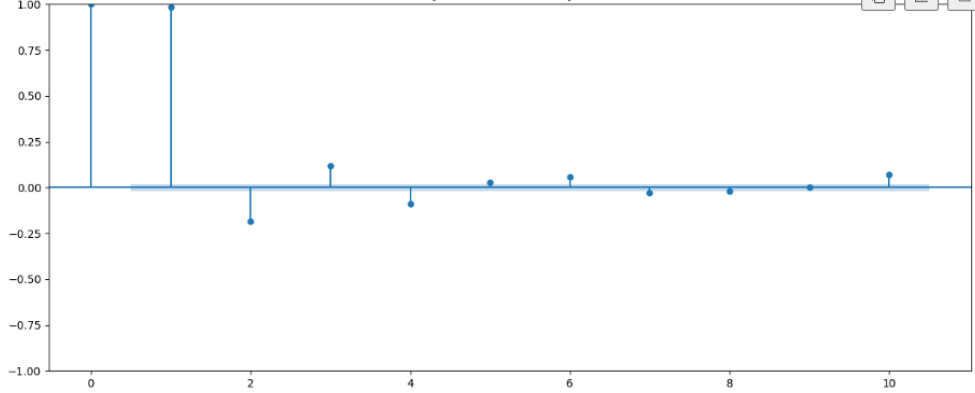
\includegraphics[width=0.9\textwidth,keepaspectratio]{figuras/imagem20.png}
	\fonte{Elaborado pelos autores com base em dados da SABESP (2025).}
\end{figure}

\begin{figure}[H]
	\centering
	\caption{Gráfico da Autocorrelação do Residuo da Vazão Jusante após remover tendência e sazonalidade.}
	\label{fig:Fig_21}
	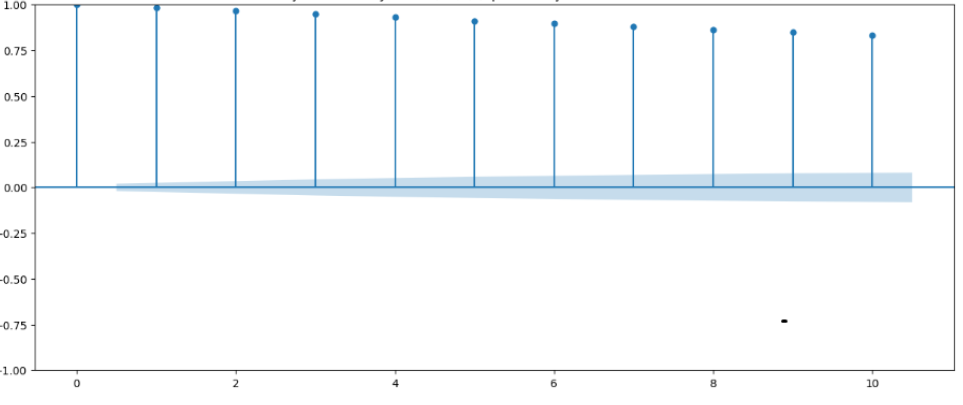
\includegraphics[width=0.9\textwidth,keepaspectratio]{figuras/imagem21.png}
	\fonte{Elaborado pelos autores com base em dados da SABESP (2025).}
\end{figure}

\begin{figure}[H]
	\centering
	\caption{Gráfico da Autocorrelação do Residuo da Vazão Jusante.}
	\label{fig:Fig_22}
	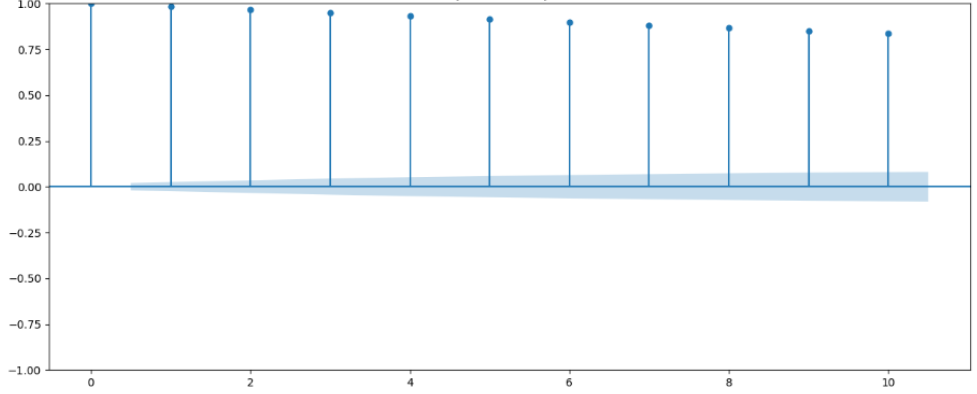
\includegraphics[width=0.9\textwidth,keepaspectratio]{figuras/imagem22.png}
	\fonte{Elaborado pelos autores com base em dados da SABESP (2025).}
\end{figure}

Analogamente, nesses gráficos de ACF e PACF da vazão jusante, o lag 1 e, talvez lag2, fazem sentido serem utilizados para realizar previsões na série temporal de vazão jusante.  

\subsection{Relação entre Variáveis}

Conforme discutido nesta seção, as variáveis analisadas podem ter relações entre si. Foi visto que a chuva e a vazão natural parecem ter uma boa relação, já que a distribuição de seus valores segue um comportamento parecido, com a vazão apresentando valores mais altos entre outubro e março, que coincide com os períodos chuvosos. Mas é notável que, o volume não acompanha essa distribuição, os períodos de cheia do reservatório estão justamente fora do período chuvoso, o que mostra que essas variáveis não influenciam imediatamente o reservatório, mas sim depois de um tempo. Primeiramente para verificar se existem relações lineares claras entre as variáveis, podemos observar a \autoref{fig:Fig_23} a seguir. 

\begin{figure}[H]
	\centering
	\caption{Matriz de Correlação entre as Variáveis.}
	\label{fig:Fig_23}
	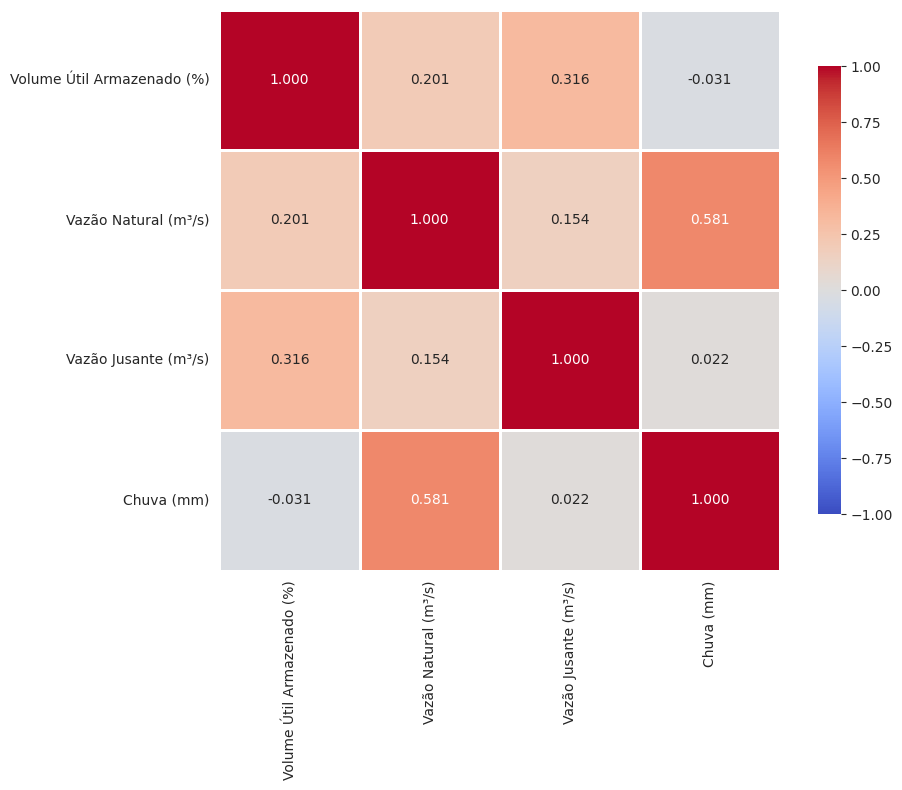
\includegraphics[width=0.9\textwidth,keepaspectratio]{figuras/imagem23.png}
	\fonte{Elaborado pelos autores com base em dados da SABESP (2025).}
\end{figure}


Através da matriz de correlação entre as variáveis, pode-se observar que existe uma relação maior da chuva com a vazão natural, do que até mesmo de ambas as variáveis com o volume útil do reservatório. Ainda assim, observa-se que as vazões apresentam sim uma relação com a variável alvo. Já a chuva, quase não possui relação linear com o volume útil, o que já era esperado após as análises feitas anteriormente, onde foi entendido que a mesma não tem efeitos imediatos sobre os reservatórios. 

Outra maneira de avaliar a relação de causalidade entre as variáveis, é observar como se comportam as séries temporais das variáveis em relação umas às outras. O gráfico da \autoref{fig:Fig_24} a seguir mostra a série temporal do volume útil e das variáveis exógenas de vazão natural, jusante e chuva. Como o objetivo principal é avaliar o comportamento das variáveis entre si, foi realizada a normalização dos dados, a fim de coloca-los na mesma escala, pois os dados originais têm magnitudes diferentes o que poderia dificultar a comparação no comportamento das mesmas.  Além disso, para que o gráfico ficasse menos ruidoso, optou-se por usar as médias móveis das variáveis ao invés dos valores diários. 

Através da análise do gráfico da \autoref{fig:Fig_24}, nota-se que a vazão natural e a chuva de fato têm um comportamento parecido, quando a chuva é alta, as vazões naturais são altas, o que sugere que a chuva tem uma ação de curto prazo sobre a vazão natural. Ainda podemos observar que, a ocorrência de valores altos na vazão natural e chuva precede o aumento do volume útil, quando há picos nessas variáveis a tendência do volume é subir, e quando os valores são baixos logo em seguida o volume começa a cair. No entanto o efeito não é imediato, embora a direção na tendência dos dados mude conforme muda o comportamento dessas variáveis exógenas, o volume não sobe abruptamente. Por fim, nota-se que ocorre o comportamento contrário quando comparados o volume útil com a vazão jusante, os picos de saída do reservatório, geralmente antecedem uma queda no volume.    

Além disso, analisando o gráfico \autoref{fig:Fig_24} a seguir, que apresenta a evolução temporal das vazões a jusante, natural e do volume, tem-se que é possível notar uma relação de áreas entre a variável de vazão natural e volume, o que é esperado no modelo físico, uma vez que a área da vazão natural se refletiria no aumento de volume caso não tivéssemos saída. É possível notar que em períodos que a vazão vem de sequências de alta como entre 2009 e 2013, o volume acompanha (com uma pequena defasagem) e em períodos de sequências de baixa, o volume cai consideravelmente, como é o caso do ano de 2015. Neste gráfico, ainda é possível notar que os picos de vazão jusante ocorreram exatamente nas altas de volume e vazão natural, o que é esperado também, uma vez que temos alta disponibilidade de água, a SABESP diminui tarifas e também disponibiliza mais água, o que faz aumentar o consumo (influenciando períodos de volume menor no futuro). 

\begin{figure}[H]
	\centering
	\caption{Evolução Temporal das Vazões a Jusante, Natural, Chuva e do Volume Útil do Sistema Cantareira entre 2000 e 2025.}
	\label{fig:Fig_24}
	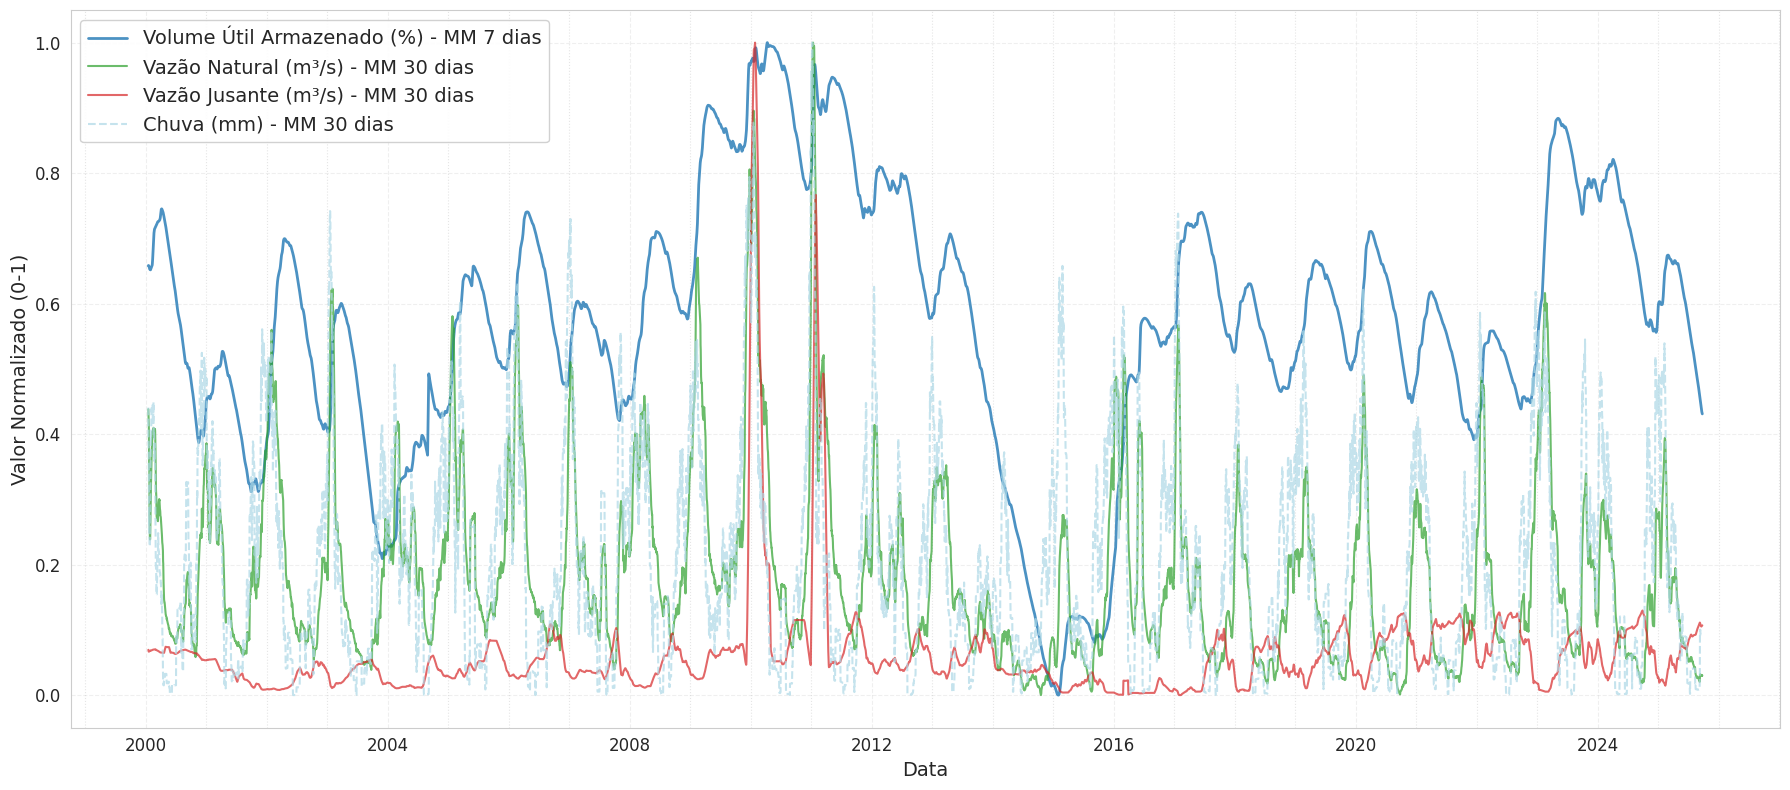
\includegraphics[width=0.95\textwidth,keepaspectratio]{figuras/imagem24.png}
	\fonte{Elaborado pelos autores com base em dados da SABESP (2025).}
\end{figure}

\section{Modelagem}

\subsection{Visão Geral do Modelo Adotado}

Conforme exposto na fundamentação teórica, foi adotada uma abordagem híbrida em cascata para previsão do volume útil (\%), essa abordagem é composta por duas etapas sequenciais:

\begin{enumerate}
\item Modelo híbrido para prever a vazão natural e vazão jusante (m³/s)
\item Um modelo de regressão supervisionada que utiliza as vazões previstas pelo módulo anterior como variável exógena para estimar o volume útil final.
\end{enumerate}

A previsão é executada sob uma estratégia recursiva multi-step. Isso significa que, durante o horizonte de teste, o modelo não tem acesso a dados reais futuros; a predição do instante $t$ alimenta as entradas (features) do instante $t+1$, essa abordagem simula fielmente um cenário operacional real e expondo o modelo ao desafio da propagação de erros ao longo do tempo.

\subsection{Modelagem das Variáveis Exógenas – Vazão Natural e Vazão Jusante}

A fim de representar adequadamente a dinâmica física do reservatório, o modelo foi expandido para prever o balanço hídrico completo, ou seja, a entrada e saída de água do reservatório. Para tanto, foram consideradas duas variáveis explicativas fundamentais: A vazão natural ($Q_{nat}$), que representa a afluência de água no reservatório, ou seja, a entrada de água, e é regida por processos hidrológicos e climáticos, como chuvas nas bacias de contribuição. E a vazão jusante ($Q_{jus}$), que representa a defluência, ou seja, a saída de água liberada para o rio ou canal a jusante, sendo uma variável influenciada tanto por regras operacionais de controle de cheias quanto por demandas de abastecimento.

Observou-se que ambas as séries temporais, embora regidas por forças distintas (fenômenos naturais vs. operação humana), ambas apresentam forte comportamento sazonal e cíclico. Dessa forma, optou-se por uma arquitetura de modelagem simétrica, sendo assim, o mesmo pipeline de decomposição e previsão híbrida descrito foi aplicado independentemente para a Vazão Natural e para a Vazão Jusante. E o processo para ambas as variáveis seguiu as seguintes etapas:

\begin{enumerate}
\item \textbf{Decomposição para extração de resíduos}: nesta etapa o objetivo foi isolar o componente cíclico não-linear. Para isso, primeiramente ajustou-se um modelo determinístico composto por uma tendência linear e termos de sazonalidade anual via Séries de Fourier. Optou-se por utilizar termos de Fourier de sazonalidade anual, através da análise do periodograma mostrado no capítulo 2, que mostra forte sazonalidade anual das vazões. O objetivo desta etapa não foi a previsão final, mas sim a ``limpeza'' da série, permitindo calcular o resíduo ($R_t$), que é a diferença entre a vazão observada e a curva matemática suave das componentes determinísticas. Este resíduo contém a informação sobre os ciclos de curto prazo, como: anomalias de seca, cheia ou alterações operacionais de descarga.

\item \textbf{Modelagem do Ciclo (Resíduo)}: O componente residual foi modelado como uma dinâmica autoregressiva local. Utilizando defasagens (lags) do próprio resíduo como preditores, foram avaliados algoritmos de aprendizado de máquina não-paramétricos, especificamente KNN (K-Nearest Neighbors) e Random Forest. A escolha desses algoritmos visa capturar padrões de dependência não-linear que modelos clássicos (como AR) falham em identificar.

\item \textbf{Reconstrução via climatologia robusta}: Um diferencial metodológico deste trabalho reside na etapa de reconstrução da previsão final. Embora a extração do resíduo tenha utilizado Fourier, a recomposição da vazão ($Q_{prevista}$) foi realizada somando-se o ciclo previsto pelo algoritmo de machine learning a uma climatologia robusta. Para cada dia, a climatologia foi calculada através das médias de valores em janelas móveis considerando 3 dias a frente e 3 dias anteriores a data analisada, removendo os outliers que estejam abaixo do percentil 10, e acima do percentil 90. Optou-se pela climatologia na reconstrução pois ela representa melhor o regime hidrológico ``médio'' esperado e é menos suscetível a distorções nas bordas da série (fenômeno de Runge), ou rigidez excessiva que os termos de Fourier podem apresentar em séries ruidosas.
\end{enumerate}

\subsection{Controle de Superestimação em Horizontes Longos: Parâmetro de Damping}

Durante a fase de experimentação, observou-se que a previsão recursiva do componente de ciclo tendia a divergir em horizontes de previsão mais longos onde ocorreu a superestimação das previsões, um fenômeno conhecido como acumulação de erro. Acredita-se que isso se deu devido à forte influência da vazão natural no volume, então se o a previsão da vazão era superestimada, na previsão do volume, observou-se um erro onde o volume mantinha a tendência de ter valores mais altos que o esperado.

Para mitigar esse efeito e garantir a estabilidade física da previsão, introduziu-se um mecanismo estratégico de amortecimento (damping). Este mecanismo atua aplicando um fator de redução (penalidade) ao ciclo previsto quando este apresenta comportamento explosivo, como por exemplo, crescimento contínuo de anomalias positivas, conforme citado acima. A ativação e a intensidade dessa lógica foram tratadas como hiperparâmetros no Grid Search, permitindo que o próprio processo de validação determinasse se a suavização da previsão resultava em ganho de performance global.

A dinâmica para decidir se o parâmetro de damping é ou não aplicado na previsão da vazão leva em conta se o valor do resíduo obtido na decomposição é maior ou menor que o último resíduo conhecido, ou seja, se a vazão está tendendo a crescer ou decrescer. Se o resíduo for maior que o anterior, a diferença entre os mesmos será um número positivo, neste caso, aplica-se uma redução de 80\% no resíduo previsto, e caso contrário, se a diferença entre os resíduos resultar em um número negativo, aplica-se uma redução de apenas 20\% no valor previsto.

\subsection{Modelagem do Volume: Regressão com Memória Curta e Exógena de Vazão}

A modelagem do volume adotou uma abordagem de regressão linear dinâmica. Essa escolha justifica-se pela própria natureza física do problema, regida pelo princípio do balanço de massa: o volume armazenado em um instante é, essencialmente, o resultado do volume acumulado no instante anterior somado ao saldo líquido de água, ou seja, o volume que entra menos o volume que sai.

Como essa relação física é predominantemente aditiva e linear, modelos de regressão simples (Linear Regression e Ridge Regression) conseguem capturar a dinâmica de enchimento e esvaziamento com alta eficiência. Diferente da etapa de vazão, evitou-se o uso de modelos de alta complexidade (como árvores profundas ou redes neurais), pois estes tenderiam ao overfitting desnecessário dado o comportamento cumulativo da série. A regularização via Ridge foi avaliada para garantir estabilidade nos coeficientes diante da colinearidade entre os lags.

\subsubsection{Engenharia de Atributos do Volume}

O vetor de características (feature vector) para o volume foi composto por:

\begin{itemize}
\item \textbf{Componente Autoregressivo}: Lag do volume em $t-1$, representando a inércia do sistema.
\item \textbf{Dinâmica de Variação}: Diferenças de primeira e segunda ordem, capturando a velocidade e aceleração de mudança de nível (enchimento/esvaziamento do reservatório).
\item \textbf{Variáveis Exógenas}: A vazão natural e a vazão jusante, previstas pelo módulo anterior. No treinamento, utiliza-se a vazão real (para aprendizado da física); na inferência, utiliza-se a vazão estimada, caracterizando o encadeamento dos modelos.
\item \textbf{Componentes Determinísticos Híbridos (Opcionais)}: Avaliou-se também a injeção direta de termos de sazonalidade e climatologia do volume como atributos auxiliares.
\end{itemize}

Nesta etapa, não foi necessária a modelagem explícita de resíduos de volume, visto que a não-linearidade do sistema já é capturada pela variável exógena de vazão, que carrega a informação do ciclo.

\subsection{Estratégia de Otimização de Hiperparâmetros (Grid Search)}

A definição da melhor arquitetura foi realizada através de uma busca em grade (Grid Search), combinando variações estruturais e paramétricas dos modelos. As principais dimensões exploradas incluíram:

\begin{itemize}
\item \textbf{Modelo de Ciclo (Vazão)}: Comparação entre a capacidade de generalização local do KNN e a robustez de ensembles do Random Forest.
\item \textbf{Parâmetros de Estabilidade}: Ativação ou desativação da lógica de damping na previsão das vazões e inclusão de termos diferenciais de primeira e segunda ordem no volume, a fim de tentar antever comportamentos de crescimento ou decrescimento do mesmo.
\item \textbf{Regularização}: Comparação entre Regressão Linear Simples e Ridge Regression para o volume final.
\item \textbf{Features Auxiliares no modelo de volume}: Realização de testes de inclusão e exclusão de variáveis (feature selection), visando verificar se o acréscimo da climatologia de volume e dos termos híbridos de Fourier trazia ganho real de desempenho à regressão final ou apenas aumentava a complexidade do modelo desnecessariamente.
\end{itemize}

Todas as variáveis numéricas foram submetidas a padronização (StandardScaler) para garantir a convergência adequada dos algoritmos baseados em distância (KNN) e regularização (Ridge).

\subsection{Avaliação do Modelo e Métricas de Desempenho}

A avaliação do modelo foi conduzida de forma compatível com a natureza temporal dos dados, evitando vazamento de informação do futuro para o passado (data leakage). Para isso, utilizou-se validação cruzada específica para séries temporais por meio de divisões sequenciais (TimeSeriesSplit), com múltiplos cortes ao longo do histórico e janela fixa de teste (horizonte) em cada divisão (fold). Em cada fold, os modelos de vazão e volume foram ajustados exclusivamente com dados anteriores e, na sequência, executou-se a previsão do volume no bloco de teste de maneira recursiva multi-step, ou seja, as predições geradas em um instante foram utilizadas para compor os atributos do instante seguinte. O desempenho foi mensurado por métricas de erro aplicadas à variável-alvo (Volume Útil Armazenado (\%)), utilizando:

\begin{itemize}
\item \textbf{MAE (Mean Absolute Error)}: que mede o erro médio absoluto, fornecendo interpretação direta em unidades do volume e robustez relativa a erros extremos.
\item \textbf{RMSE (Root Mean Squared Error)}: que mede a raiz do erro quadrático médio, penalizando mais fortemente grandes desvios e sendo útil para comparar configurações quando se deseja reduzir erros de maior magnitude.
\end{itemize}

Para cada combinação de modelos e hiperparâmetros do grid search, as métricas foram calculadas em todos os folds e agregadas por média, adotando-se o menor erro médio (com ênfase em RMSE e apoio do MAE) como critério para seleção da configuração final.

Outros modelos clássicos como ARIMA/SARIMAX foram considerados e avaliados, porém apresentaram desempenho inferior ao obtido pela estratégia de decomposição da vazão + modelagem do ciclo por ML + regressão do volume com variável exógena, especialmente no contexto de previsão recursiva. Por esse motivo, optou-se por concentrar o desenvolvimento e a tunagem na abordagem híbrida descrita acima, que demonstrou melhor capacidade preditiva no conjunto de dados avaliado.


	
	% 4 - Conclusão
	% ----------------------------------------------------------
\chapter{Conclusão}
% ----------------------------------------------------------

O presente trabalho cumpriu seu objetivo central de aplicar, na prática, os conhecimentos teóricos adquiridos, consolidando-os em uma solução de ciência de dados com arquitetura produtiva. Ao integrar conceitos de Engenharia de Software e Hidrologia, a ferramenta desenvolvida mostrou-se eficaz no auxílio à gestão dos recursos hídricos do \acrshort{SC}, cuja posição estratégica no abastecimento da maior metrópole da América do Sul reforça a pertinência do tema. Em um cenário marcado por mudanças climáticas e eventos extremos, a transição de uma gestão reativa para uma abordagem preventiva baseada em dados ultrapassa a inovação tecnológica, configurando-se como uma necessidade premente de segurança hídrica e social. 

No que tange à modelagem preditiva, a abordagem híbrida em cascata apresentou desempenho superior às técnicas puramente estatísticas, como \acrshort{SARIMAX}, e aos modelos de "caixa-preta" (Deep Learning isolado). Ao desacoplar os componentes determinísticos (tendência e sazonalidade) dos estocásticos (ciclos e resíduos), garantiu-se não apenas uma acurácia robusta com \acrshort{RMSE} médios entre 2,1 e 2,2 nos testes de validação, mas principalmente a explicabilidade do modelo. Essa característica é vital para a tomada de decisão, pois permite ao \acrshort{SABESP} discernir se uma oscilação no volume se trata de um movimento sazonal esperado ou de uma anomalia crítica, conferindo a confiabilidade estatística necessária para embasar ações de mitigação. 

Visando uma arquitetura produtiva, a infraestrutura foi alicerçada inteiramente em serviços de computação em nuvem do \acrshort{AWS} sob o paradigma serverless. A orquestração de serviços como \acrshort{AWS} Lambda, \acrshort{ECS} e Step Functions resultou em um pipeline de MLOps automatizado e escalável, dispensando investimentos massivos em hardware físico (on-premise) ou infraestruturas muito robustas usadas em projetos necessariamente escaláveis. Essa estrutura assegura a operação contínua do sistema, que realiza coletas e inferências autônomas, transformando dados brutos em inteligência capaz de antecipar a transição para faixas de risco, como o limiar de 30\% do volume útil. 

Sob a ótica financeira, a solução comprovou sua sustentabilidade. O custo operacional (\acrshort{OPEX}) da estrutura em nuvem mostra-se irrisório se contrastado com os prejuízos potenciais de uma crise hídrica, que historicamente impõe perdas bilionárias à indústria, ao agronegócio e à saúde pública. Valida-se, assim, a premissa de que o "custo da prevenção" é infinitamente inferior ao "custo do desastre", confirmando a viabilidade econômica do projeto frente aos imensuráveis benefícios sociais de se evitar um colapso no abastecimento. 

Em suma, este trabalho deixa como legado uma base sólida para a modernização da gestão hídrica. Para trabalhos futuros, sugere-se o desenvolvimento de interfaces visuais interativas (dashboards) e o estabelecimento de parcerias técnicas para enriquecer o modelo com novas variáveis exógenas. Conclui-se que a solução cumpre seu papel acadêmico e social, entregando valor real ao alinhar rigor técnico e viabilidade financeira na proteção de um dos recursos mais essenciais à vida. 

\section{Próximos Passos}

Avaliamos para trabalhos futuros a possibilidade de disponibilizar os dados por meio de visualizações gráficas interativas como um dashboard em streamlit, para que a operadora tome suas próprias conclusões de forma mais facilitada e possa comparar modelos de forma mais rápida e fluida.  

Além disso, consideramos que pode ser válido uma participação mútua com o \acrshort{SABESP} para tentar, com o conhecimento especializado do negócio por parte dela, incluir novas variáveis e implementações que deixem o modelo mais robusto. 

Ademais, é interessante fazer uma análise mais detalhada para entender as influências das variáveis e identificar pontos que podem fazer o modelo errar ou propagar erros, isto é, explorar mais a explicabilidade dos modelos de modo a melhorar modelos futuros.  
	
	
	% Elementos pós-textuais
	\postextual
	
	
	% Referências bibliográficas
	\begingroup
	    \printbibliography[title=REFERÊNCIAS]
	\endgroup
	
	
	
	%Reconfiguração do título para apêndices e anexos
	 \renewcommand{\ABNTEXchapterupperifneeded}[1]{#1} 
	\makeatletter
	\settocpreprocessor{chapter}{%
      \let\tempf@rtoc\f@rtoc%
      \def\f@rtoc{%
      \texorpdfstring{{\tempf@rtoc}}{\tempf@rtoc}}%
      }
    \makeatother
	
	
	% Apêndices
    %\begin{apendicesenv}
    	%\partapendices* 
    	%\input{pos_textual/apendice_a}
    %\end{apendicesenv}

    % Anexos
    %\begin{anexosenv}
    	%\partanexos*
    	%\input{pos_textual/anexo_a}
    %\end{anexosenv}

\end{document}